% !TeX spellcheck = en_GB
\documentclass[11pt,a5paper,twoside]{book}
%format A5
%\usepackage[top=25mm, bottom=20mm, outer=20mm, inner=25mm]{geometry}
%Format Royal
\usepackage[paperwidth=156mm, paperheight=234mm,top=25mm, bottom=20mm, outer=20mm, inner=25mm]{geometry}
%\usepackage{fontspec}
\usepackage[utf8]{inputenc}
\usepackage{CJKutf8}
%\usepackage{xeCJK} 
%\setCJKmainfont{AR PL UMing TW MBE}
%\setCJKsansfont[BoldFont=FandolHei-Bold.otf]{FandolHei-Regular.otf}
%\setCJKmonofont{FandolFang-Regular.otf}
%\newCJKfontfamily\kaiti{FandolKai-Regular.otf}
\usepackage{makeidx}
\usepackage{graphicx}
\usepackage[hidelinks]{hyperref}
%Restricts floats within section
%\usepackage[section]{placeins}
\usepackage{placeins}
%Subfigures
\usepackage{subfigure}
%Header and footer control
%\usepackage{fancyhdr}
%\pagestyle{fancy}
%Verbatim and multi-line comments
\usepackage{verbatim}
\usepackage[english]{babel}
%Caption control
\usepackage[font=small,format=plain,labelfont=bf,labelsep=endash,textfont=up]{caption}
\captionsetup{figurename=Fig.}
%Include des macros Pinyin pour traitement de-macro avant pandoc ou tex4ebook
\usepackage{Pinyin-private}
\usepackage[abs]{overpic}
\usepackage{color}
\usepackage{anyfontsize}
%Pour les unités physiques, kg, g, cm, etc.
\usepackage[squaren,Gray]{SIunits}
%=============================================================
\title{{\Huge \TAIJIJIAN{}\\}{\huge \Taiji{} sword fencing}}
\author{{\large Frédéric Plewniak}}
\makeindex
\begin{document}
\newcommand{\fiche}[1]{}
\setcounter{secnumdepth}{0}
%\renewcommand{\chaptermark}[1]{ \markboth{#1}{} }
\renewcommand{\sectionmark}[1]{ \markright{#1}{} }
%Set the level of sections in table of contents
\setcounter{tocdepth}{1}
\frontmatter
\begin{titlepage}
%\setcounter{page}{0}
%\newgeometry{top=0mm, bottom=0mm, outer=0mm, inner=0mm, hoffset=-6mm,voffset=0mm}
%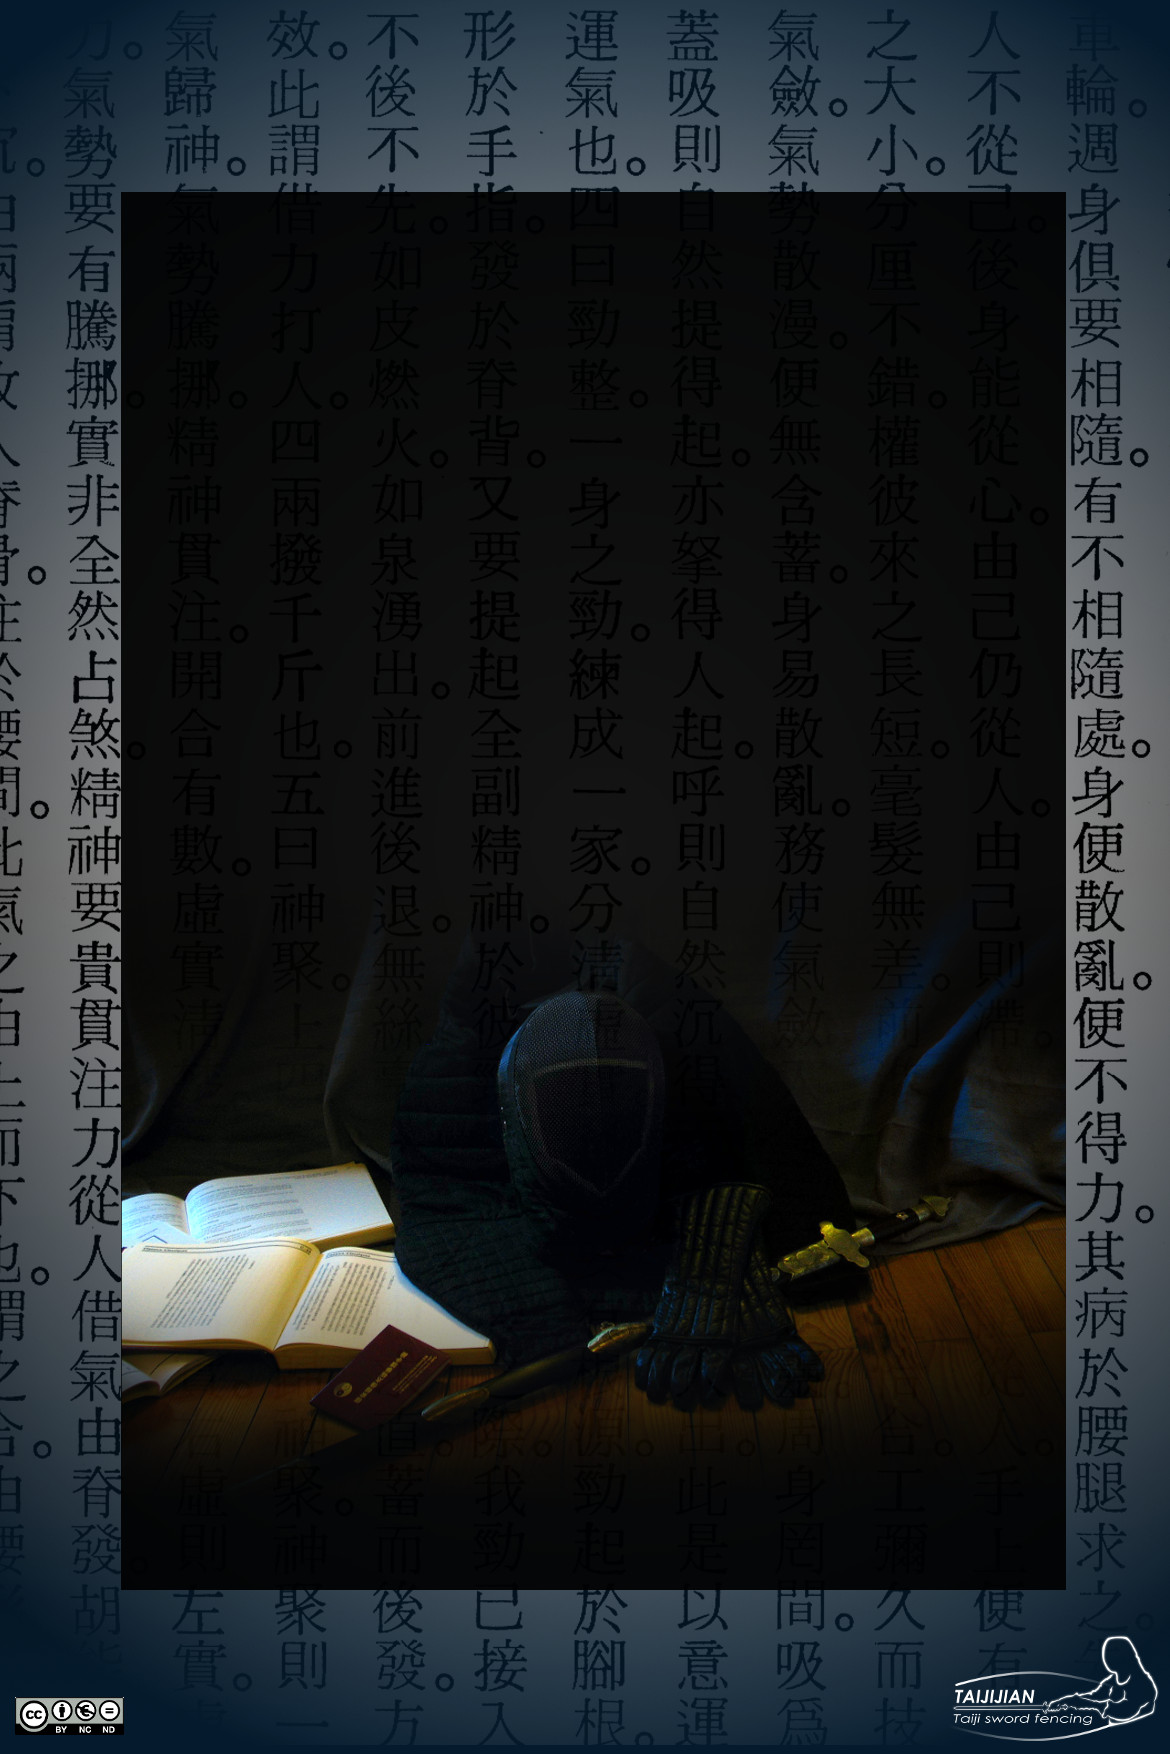
\includegraphics[width=\paperwidth]{../../Images/CouverturePDF_Royal}
\setlength\unitlength{1mm}
\newgeometry{top=0mm, bottom=0mm, outer=0mm, inner=0mm, hoffset=-6mm,voffset=1mm}
\begin{overpic}[width=\paperwidth]%
{../../Images/CouverturePDF_Royal}
\put(28,180){\color{white}{{\upshape\fontfamily{ppl}\fontseries{b}\fontsize{50}{60}\selectfont \TAIJIJIAN{}}}}
\put(30,165){\color{white}{{\upshape\fontfamily{ppl}\fontseries{l}\fontsize{32}{30}\selectfont \Taiji{} sword fencing}}}

\put(70,25){\color{white}{{\scshape\fontfamily{pbk}\fontseries{l}\fontsize{20}{20}\selectfont Frédéric Plewniak}}}
\end{overpic}
\thispagestyle{empty}
\restoregeometry
\end{titlepage}
\maketitle
\thispagestyle{empty}
\setcounter{page}{0}
% !TeX spellcheck = en_GB
\scriptsize
\par\vspace*{\fill}
\begin{center}

\includegraphics[height=2em]{../../Licence/by-nc-nd}

\copyright{} Fr\'{e}d\'{e}ric Plewniak 2014-\the\year
\end{center}

\begin{center}
This work is licensed under the Creative Commons Attribution-NonCommercial-NoDerivatives 4.0 International License. 

http://creativecommons.org/licenses/by-nc-nd/4.0/legalcode
\end{center}
\medskip
\subsubsection{{\footnotesize You are free to:}}
\paragraph{}\textbf{Share} \textendash{} copy and redistribute the material in any medium or format
\paragraph{}The licensor cannot revoke these freedoms as long as you follow the license terms.

\subsubsection{{\footnotesize Under the following terms:}}
\begin{itemize}
\item{\textbf{Attribution}  \textendash{} You must give appropriate credit, provide a link to the license, and indicate if changes were made. You may do so in any reasonable manner, but not in any way that suggests the licensor endorses you or your use.}

\item{\textbf{NonCommercial}  \textendash{} You may not use the material for commercial purposes.}

\item{\textbf{NoDerivatives}  \textendash{} If you remix, transform, or build upon the material, you may not distribute the modified material.}

\item{\textbf{No additional restrictions} — You may not apply legal terms or technological measures that legally restrict others from doing anything the license permits.}
\end{itemize}

\subsubsection{ {\footnotesize Notices:}}

\paragraph{}You do not have to comply with the license for elements of the material in the public domain or where your use is permitted by an applicable exception or limitation.
\paragraph{}No warranties are given. The license may not give you all of the permissions necessary for your intended use. For example, other rights such as publicity, privacy, or moral rights may limit how you use the material.
\clearpage
\normalsize
\tableofcontents
\listoffigures
% !TeX spellcheck = en_GB
\chapter{Preface}

\paragraph*{}
In most styles and schools, \Taijijian{} is studied quite exclusively as routines and most of the time without much consideration for its martial roots. 
Although we see now a growing interest in two-person drills, mainly in the form of sticking sword exercises, martial applications are very rarely demonstrated and are often limited to martial explanations and justifications of the routine movements. 
What may be truly called \Taijijian{} fencing is even more rarely evoked or practised.

\paragraph*{}
The present work is an attempt to bridge the gap between \Taiji{} sword form practice and \Taijijian{} fencing.
It is the result of nearly fifteen years of research and experimentation,
trying to uncover the martial dimensions of \Taijijian{}, from fencing basics and martial applications of the form through free sparring with respect for the \Taiji{} principles.
The sources of this work are rooted in the \Yangjia{} \Michuan{} \Taijijian{} tradition as transmitted by Master
Wang Yen-nien, and mainly the \Kunlun{} sword routine, also known in
this style as the \emph{Old Sword Form}.
Historical European fencing from the XIII\textsuperscript{th} to the XVIII\textsuperscript{th} centuries also provided valuable inspiration.
This might seem strange at first sight, but actually, European fencing treatises of past centuries do remind sometimes of our \Taiji{} classics and a good deal of European techniques present striking similarities to those found in \Taiji{} sword forms.
In particular, applying to the \Kunlun{} routine form the
concept of \emph{fencing phrase} which describes fencing actions as if
it were a conversation, allowed me to discover convincing martial
applications for most movements of this form.
In all those cross-cultural experimentations though, my guides have always been the \Taiji{} principles, \Taiji{} classics and Master Wang Yen-nien's precepts.
I did not have the luck to be a direct student of Master Wang, however his
books and my notes from the few workshops I could attend contain a
wealth of enlightening information.
I also owe my teachers, who had been his direct students and truthfully transmitted his teachings, an immense debt of gratitude.
I do believe therefore that the sword techniques and notions you will find in these pages can confidently be considered as appropriate \Taiji{} sword techniques, respectful of principles, even though some may have been elucidated thanks to unrelated but nonetheless convergent sources.

\paragraph*{}
This is still a work in progress and in constant evolution.
I do not pretend to hold the absolute truth nor to have succeeded in
reconstructing genuine historically accurate \Taiji{} sword techniques.
Actually, I do not care, this was not my goal.
The only thing that really matters to me is how this work can help improving \Taijijian{} practice and the comprehension of \Taiji{} principles.
Today, I have the feeling that this work is consistent at last and worth sharing with all those interested no matter the style they practice.

\paragraph*{}
As I considered publishing my work, doing so for free in the form of a
web site soon became self-evident.
It would ensure a wide diffusion while at the same time avoid all the hassle of book printing.
Another important reason was that, before you can actually appear in print, you have to write the book from beginning to end first.
A web site, on the opposite, can start with partial content and may be easily updated and augmented gradually with new material.
Last but not least, a web site would allow better integration of various media such as video.
However, since off-line reading might be desirable sometimes, downloadable
versions will also be made available in epub and PDF formats.
The choice of the Creative Commons BY-NC-ND licence was also an evident response to the same concerns.
Derivative works and commercial distribution are not allowed without my prior consent but unmodified content may otherwise be freely redistributed provided proper credit is given.

\paragraph*{}
Hoping that this work will prove itself useful to practitioners and may
spark off new vocations.

\begin{flushright}
Fr\'{e}d\'{e}ric Plewniak, January 2014.
\end{flushright}

\mainmatter
\part{Generalities}
% !% !TeX spellcheck = en_GB
\chapter{The Chinese sword}\label{ch:chinesesword}

Broadly, a sword can be defined as a cutting and thrusting edged weapon with a blade at least as long as the arm and a short handle.

There is archaeological evidence of the use of swords dating back as far as the Bronze Age, both in the Occidental world and in China.

From these early times to the beginning of the XX\textsuperscript{th} century when they ceased to be used for combat, swords have evolved in parallel with fighting techniques and strategies.
The swordsmanship of any particular historical period was adapted to the currently available types of swords while being at the same time deeply rooted in its social and cultural context.

Thus, \Taijijian{} adopted the kind of straight double-edge swords, or \Jian{}, that were being commonly used at the time by every Chinese martial art.
Although there had never been in historical times any sword specifically tailored for the practice of \Taijijian{}, this Chinese double-edged sword is nowadays often abusively denoted by the term \Taiji{} sword.

\section{From the battlefield to the public park}
I will not get deep into historical considerations about Chinese swordsmanship. Others, more knowledgeable on the subject than I am, have already published works more accurate and extensive than anything I could write here.
For a more detailed account, I can only refer the interested reader to Peter Lorge's book \textit{Chinese Martial Arts: from Antiquity to the Twenty-First Century} and Scott Rodell's \textit{Chinese Swordsmanship}.

After having dominated Chinese battlefields until the late XIX\textsuperscript{th} and early XX\textsuperscript{th} century, edged weapons were eventually superseded by modern firearms and artillery. Practical sword fencing rapidly declined during the early XX\textsuperscript{th} century.
\ChenWeiming{}, in his book \textit{Taiji sword}, first published in 1928, mentions fencing only to say that \YangChengfu{} never taught any sword fencing set, and that he would himself write another sword book when he becomes proficient in it. As far as I can tell, this book was never written.
During the 1930s and 1940s, Chinese sword manuals lament that this ancient art was almost completely lost. 

At the same period, as China was falling under the influence of Western Empires, invaded by Japanese troops, then ravaged by the Civil War, Chinese martial arts were becoming symbols of national pride while gradually turning into disciplines for physical education, health and self cultivation.

Boxing and wrestling soon overtook weapon training, which was reduced to a mere form practice and a complement to unarmed martial arts. 
The primary goal of Chinese martial arts instructors was not to train combatants any more, but to strengthen their nation by invigorating their fellow compatriots while expressing the superiority of Chinese tradition.
Practical fencing was not sought, but swift and athletic demonstrative movements started to be favoured over effectiveness in combat.
Light swords with extremely flexible blades were more and more commonly used and somewhat became the norm.

Though there is to my knowledge no written mention of a martial art called \Taijiquan{} before the XIX\textsuperscript{th} century, the \Taiji{} principles had certainly been around for quite a long time when they were gathered into a whole coherent martial system, supposedly by the \Chen{} family of \Chenjiagou{}, and later formalised by scholars in the texts we know today as the \Taiji{} Classics.

The general \QiJiguang{} (1527\textendash{}1587), as early as the XVI\textsuperscript{th} century, cites in his \textit{New Manual on Military Efficiency} technique names that should sound familiar to every \Taijiquan{} practitioner.
It is unclear, however, whether \QiJiguang{} was actually writing about \Taijiquan{}, or its ancestor, or whether it was a mere coincidence or a later reuse of technique names.

In any case, it is generally admitted that \Taijiquan{} emerged and developed between late XVII\textsuperscript{th} and the  XIX\textsuperscript{th} century, during the \Ming{} and \Qing{} dynasties.

The \Yangjia{} \Michuan{} style, root of the present work, was created by \Yang{} \Luchan{}, presumably during the first half of the XIX\textsuperscript{th} century.
I have no clear evidence that the \Yangjia{} \Michuan{} \Kunlun{} sword form originates from this period, but the rhymes that describe the movements seem to point to a rather ancient origin.
\QiJiguang{}'s treatise contains indeed a collection of such rhymes that were used as mnemonics for routine practice.

Originally, forms had been used for training troops of soldiers to manoeuvre and fight in unison. However, as early as during the \Tang{} dynasty, training sessions shifted towards a sort of martial spectacle, not only for military power display, but also as a mere entertainment. 
In order to please spectators who often were not martial artists themselves, forms increasingly incorporated demonstrative techniques that would be much more spectacular or aesthetic than truly effective.
This interest for martial spectacles has persisted to this day in literature, Chinese Opera, cinema, and, of course, in the unavoidable demonstrations performed during Martial Arts gatherings.

Nowadays, like any other Chinese martial art, \Taijijian{} has definitely left the battlefield for the public park and sword training is fortunately anything but a preparation to combat.

Despite their undeniable aesthetic dimension, however, traditional \Taijijian{} forms were originally designed to develop martial skills based on the \Taiji{} principles, effectively using swords whose weight, dimensions and balance achieved a compromise between cutting power, thrusting precision, and swift movements.

\section{Anatomy of the \Jian{}}
The figure \ref{fig:sword_parts} shows the disassembled parts of a \Jian{}, or Chinese double-edged sword, typical of the \Ming{} and \Qing{} dynasties. 

\begin{figure}[ht]
\centering
	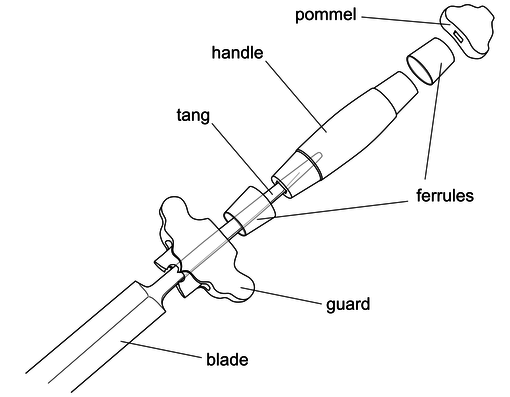
\includegraphics[width=0.69\textwidth]{../../Images/SwordParts/SwordPartsEn.pdf}
	\caption[Sword parts]{Sword parts: The double-edged straight blade is extended by the tang, traversing the guard, handle and pommel where it is secured by peening. The two ferrules are metallic rings preventing the extremities of the handle from splitting open. The guard protects the hand holding the sword. Usually made of bronze or a similar metal, it is hollow and open towards the front. The handle, generally made of wood, is spindle-shaped and sometimes covered with a string, leather or ray skin in order to prevent the grip from slipping.
The pommel, made of the same metal as the guard plays a crucial role in the sword's balance and behaviour by counterbalancing the weight of the blade.}
	\label{fig:sword_parts}
\end{figure}

The main particularity of the \Jian{}'s blade is its very gradual taper with nearly parallel cutting edges. From approximately 3 or \unit{4}{\centi\meter} at the base, the blade width decreases only to 2 or \unit{3}{\centi\meter} near the tip, where the edges curve rapidly into a sharp point.
With a blade length of 70 to 80 cm, the angle between both edges is hardly noticeable, in sharp contrast to the more triangular shape of many European mediaeval swords

Traditionally, the section of the blade could be either lenticular or diamond-shaped with a clearly marked central ridge.
Some blades could also have a \index{fuller}fuller, which is often wrongly called \emph{blood groove} because of the legend pretending that its role was to let the blood flow out of the wound.
Another delusion about the fuller is that it would prevent the blade from being stuck in the wound because of a supposed phenomenon of suction or a hypothetical contraction of the severed muscles.
I must say that I do have serious doubts about the capacity of a wounded muscle to contract significantly around a sharp blade without suffering any further damage. And assuming it could, there is certainly no reason why the blade could not cut its way out quite easily.

The truth is far less enthralling: a \index{fuller}fuller simply makes a lighter blade without compromising its solidity. Of course, the easiest way to reduce blade weight is to make it thinner. This, however, is limited by the resulting increase in flexibility, which might not be desirable beyond some degree. It also flattens the edge geometry, which might in turn affect edge durability. The \index{fuller}fuller permits a lighter blade without at the same time affecting flexibility and edge geometry.
For example, a fuller 1 cm wide and 2 mm deep, running along two thirds of a 75 cm blade with a lenticular section, would have a volume of approximately \unit{10}{\centi\meter\cubed}. As steel density ranges from \unit{7.3}{\kilo\gram \per \deci\meter\cubed} to \unit{7.8}{\kilo\gram \per \deci\meter\cubed} depending on its composition and heat treatment, such a fuller on each side of the blade would reduce its weight by about 150 g without affecting the profile of its edges. (see figure \ref{fig:blade_section}) 
This could certainly make a difference considering that a lighter blade would also mean lighter fittings. Thus, this fuller would allow a swordsmith to make a 900 g sword, the typical weight of a historical \Jian{}, with the same edge profile and blade length as a non-fullered sword weighing over 1 kg.

\begin{figure}[ht]
\centering
	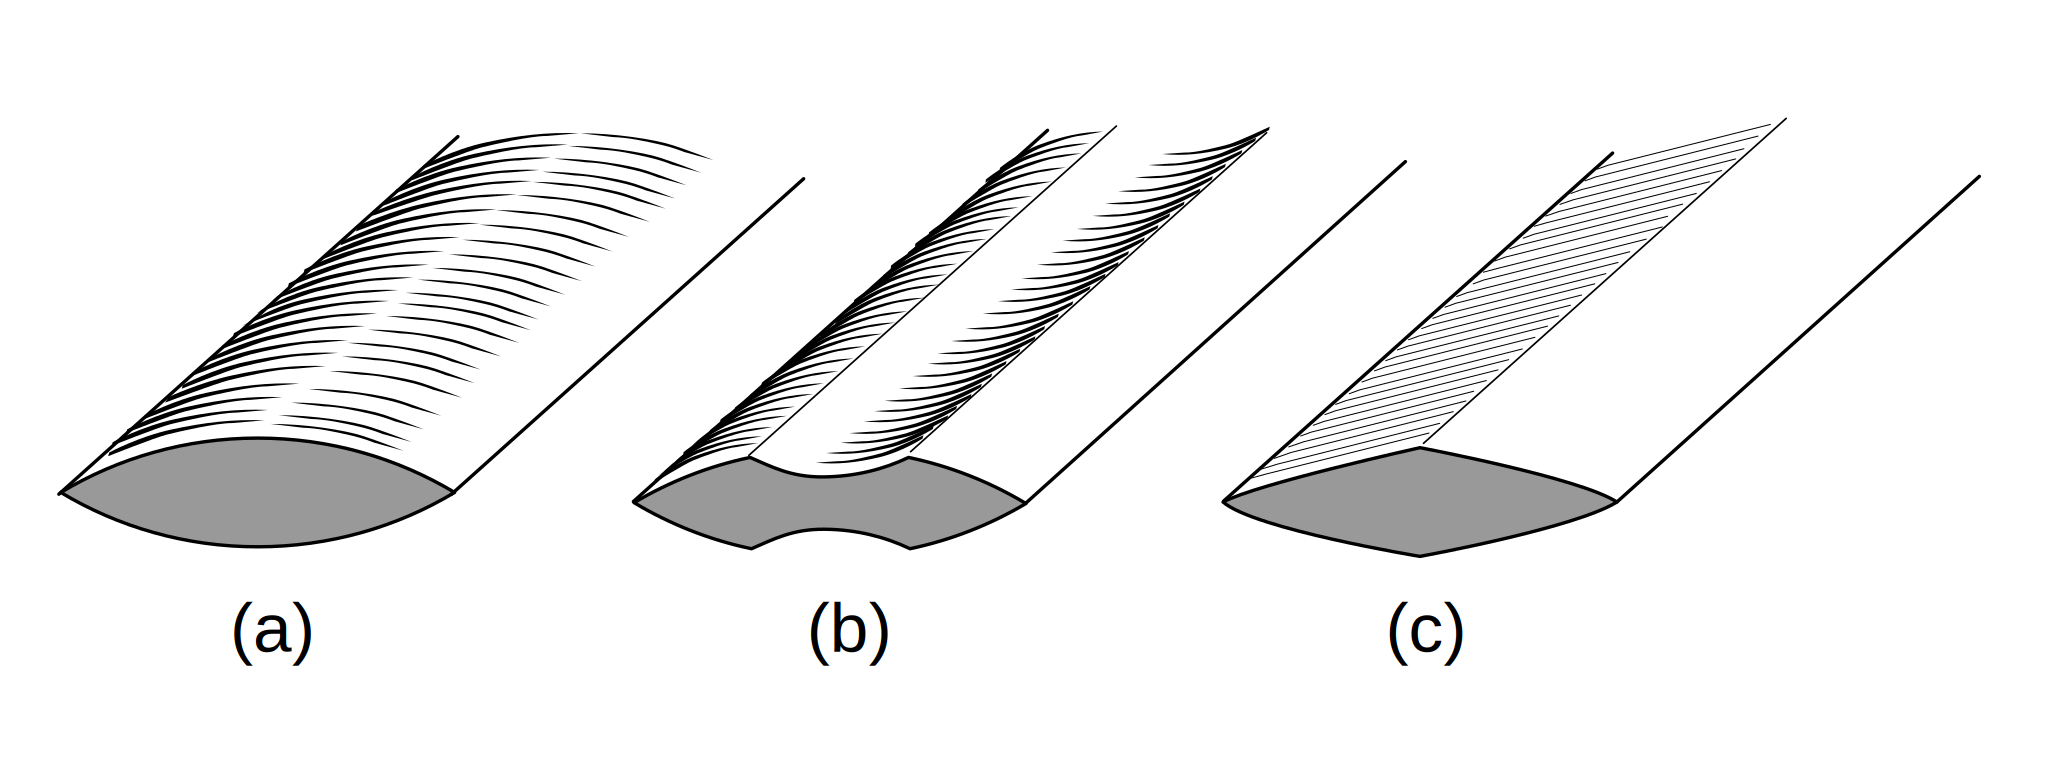
\includegraphics[width=0.69\textwidth]{../../Images/BladeSection/BladeSection.pdf}
	\caption[Blade section]{Blade sections: (a) Lenticular, or apple-seed. (b) This fullered lenticular blade has the same edge profile as the blade shown in (a), but it is significantly lighter thanks to the fuller. (c) Diamond-shaped.\\
	NB: for a clearer picture, the blade thickness has been exaggerated on this figure.}
	\label{fig:blade_section}
\end{figure}

If the blade profile may have an effect on edge durability, the kind of steel the blade is made of will also affect edge strength.  
If the steel is too soft, edges may bend and become dull after only a few cuts. Hardened steel is necessary for keeping the edges sharp, but it is also brittle and a blade cannot be made exclusively of hard steel. 
A compromise had thus to be found between blade hardness, softness and elasticity.

Note that elasticity is not a synonym for flexibility: it is the capacity of the blade to bend and return to its original shape. If the limit of elasticity is exceeded, the blade is permanently deformed or breaks. 

The blade must be hard enough for keeping its edges and at the same time sufficiently resilient and elastic so as to sustain strong blows and shocks without breaking nor taking an unwanted bend.
%Blade elasticity will also help dissipate the energy from shocks and strong blows. Vibrations, vibration node in the handle

Steel is basically a mixture of iron and a very small proportion of carbon, between 0.1\% to 2\%. It can also be alloyed with a small amount of other metals such as chromium, nickel, manganese, etc.
Even in such small quantities, these elements may, in conjunction with heat treatment, dramatically change steel mechanical properties.

\index{quenching}Quenching is a process consisting in heating the blade at a high temperature and then cooling it down rapidly by immersion into water. 
Following this treatment, steel assumes a particular crystal structure which makes it harder, but also more fragile.
Furthermore, since it is impossible to cool instantly and homogeneously the whole blade at once, quenching also creates persistent tensions in the metal that may greatly weaken the blade.
To release these constraints without reverting the hardening effect of quenching, it is possible to apply a second heat treatment, called tempering\index{tempering}. It consists in reheating the blade at a lower temperature before leaving it to cool down naturally, so as to recover sufficient resilience.

An alternative to these two successive treatments is the technique called \index{tempering!differential tempering@\textit{differential tempering}}differential tempering. Well-known for being the traditional way of Japanese swords making, this technique was originally used also in China.
In differential tempering only the edges are exposed to the quenching treatment thanks to the application of clay onto the core of the blade, which is thus protected from the heat shock and remains elastic while the edges are hardened.

In mediaeval Europe, hardened edges were sometimes welded on a soft core. As far as I know, this technique was used in China only for broad swords.
Chinese straight swords traditionally had a three-layer pattern called \SanMei{}. The blade was made of three layers of steel welded together: a thin central one of hardened steel forming the edges, and two layers of softer steel or iron protecting the former from being shattered by strong blows and providing the blade with an elastic structure.

\section{Balance and dynamic properties}\index{balance}
A sword's balance is traditionally expressed by the location of its \index{centre of gravity}centre of gravity (COG) also known as the centre of inertia. For a \Jian{}, the COG is usually located about 10 to 20 cm in front of the guard, as measured from the forward end of the handle.

But I think that there is usually too much emphasis on the COG location. Although the COG does play an important role in sword handling it is far from being the main feature affecting sword's tractability. While the COG of an object describes its static balance and how it responds to the global application of a physical force independently of its actual shape, dynamic rotational properties also depend on mass distribution and shape. This is why a rod and a ball do not handle the same at all although both have their COG located at their geometric centre.

Dynamic rotational properties are thus even more essential and determine how the sword feels when wielded, how it moves, rotates and responds to the actions exerted on the handle. As a matter of fact, it is not uncommon to find swords with a COG located at the same distance from the handle but feeling completely different when wielded. 

But measuring the physical property relating to sword rotational dynamics, the momentum of inertia, is not that easy, and even when it has been measured, interpreting this scientific value in terms of practical sword handling is far from being straightforward. 

One way of accurately measuring the momentum of inertia of a sword is the pendulum test which consists in measuring its natural oscillation period around an axis located at a given distance of the COG. After a bit of maths, you end up with a figure that will not tell you much without any reference, to be honest. More research is definitely needed here.

A much easier way to examine the dynamic properties of a sword is the waggle test. Although it is much less accurate, it has the advantage of providing some indication on how these properties actually relate to how the sword will react to your actions on the handle.

To perform this test, hold the sword lightly by the handle between your thumb and forefinger, and then wave it smoothly sideways. You will notice a point somewhere in the blade that does not move: this is the\index{pivot point} pivot point relative to the place of the handle where you were holding the sword (see figure \ref{fig:pivot_points}).

\begin{figure}[ht]
\centering
	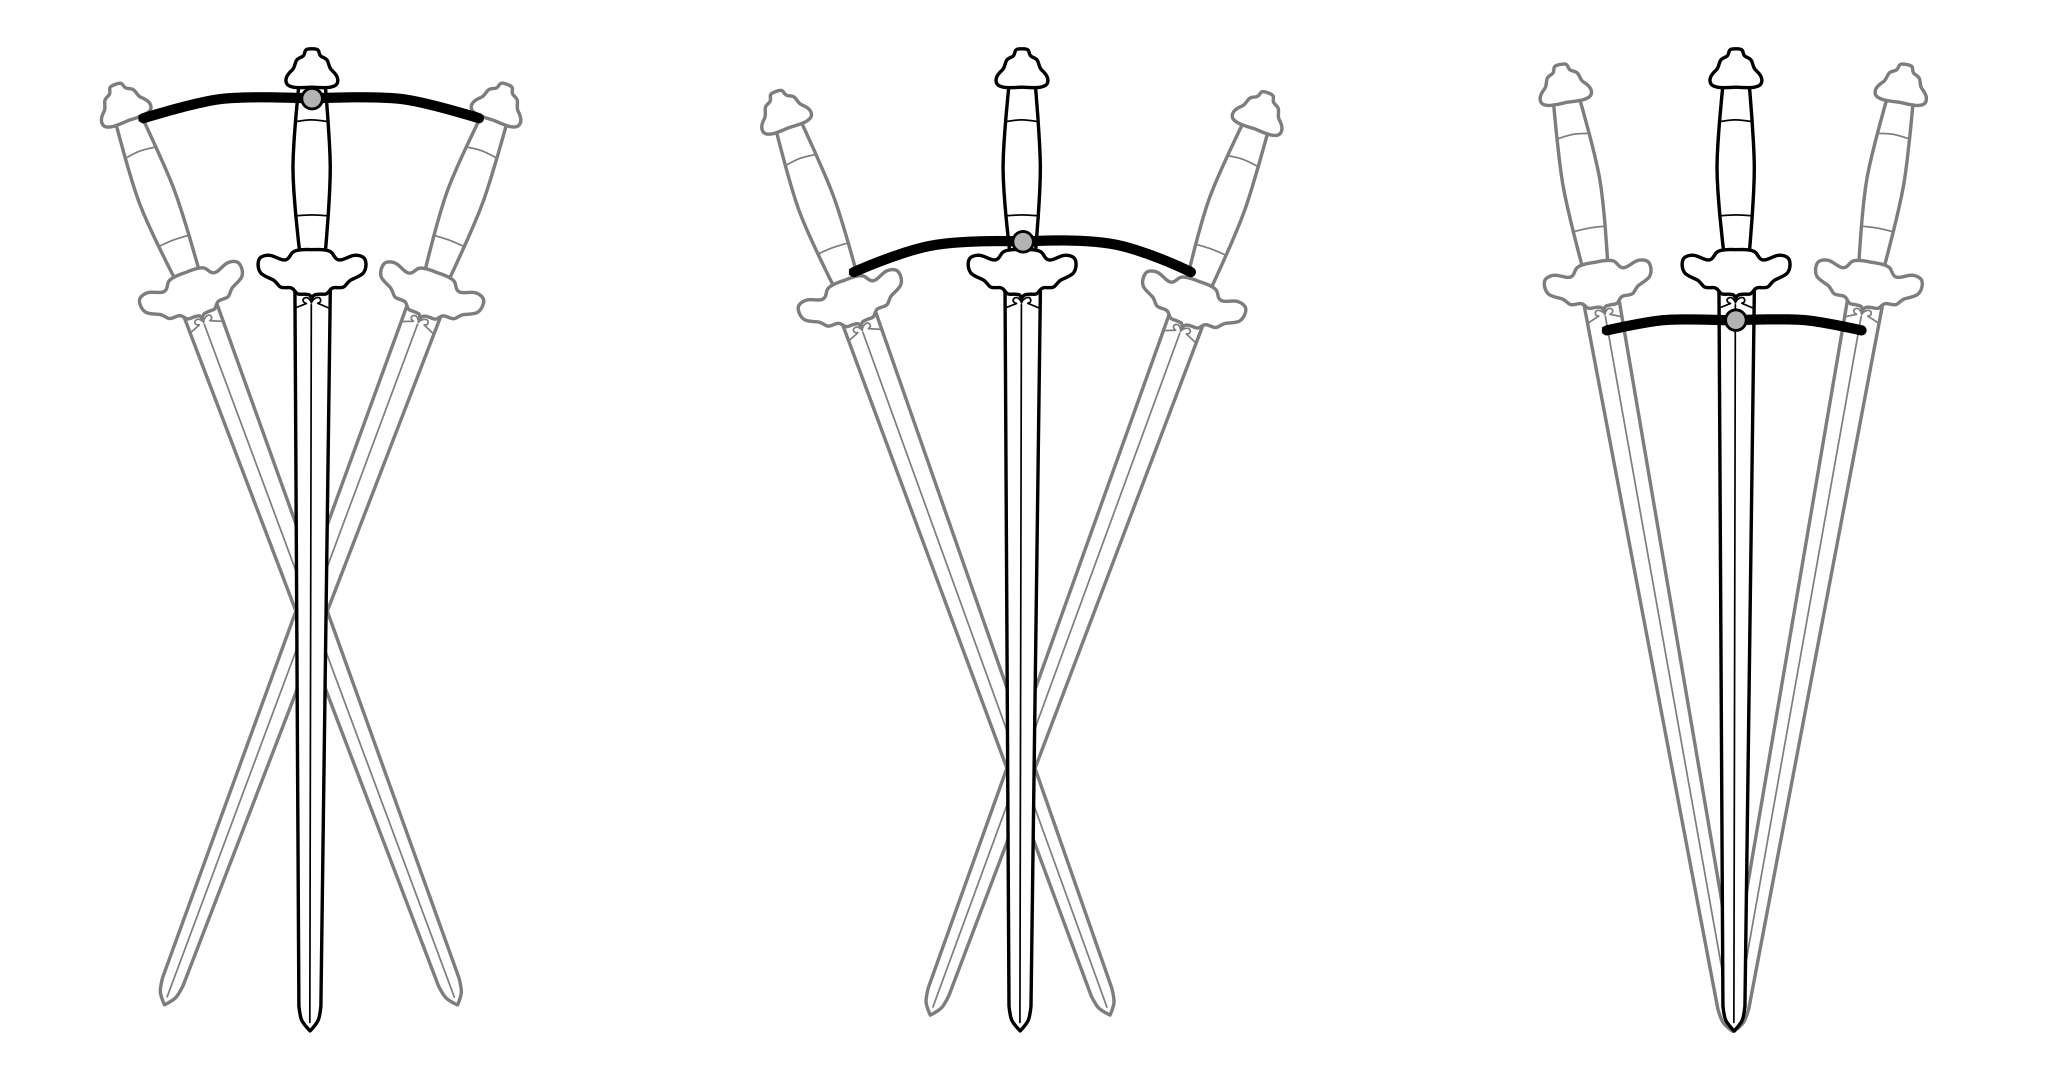
\includegraphics[width=0.80\textwidth]{../../Images/PivotPoints/PivotPoints.pdf}
	\caption[Pivot points]{A pivot point is the natural centre of rotation of the sword relative to the place and direction of an action applied to the handle. If the sword is held near the pommel and waved sideways, the pivot point is close to the centre of the blade (left). Holding the sword close to the guard will move the pivot point further down the blade towards the tip (middle). To place the pivot point at the tip of the blade for this sword, a lateral action must be applied about an inch in front of the guard (right). Although this may seem an inconvenience, a proper adjustment of the grip and a slanted action on the handle nonetheless allows the control of this point. Furthermore, this may also help to keep the blade tip in line when thrusting while controlling the opponent's blade with the guard.}
	\label{fig:pivot_points}
\end{figure}

Changing the position of the fingers on the handle will move the pivot point to another location. When wielding a sword, it is thus possible to control the location of the sword's centre of rotation by adjusting the place and direction of the action applied by the grip on the handle.

The pivot points relative to the hilt, are usually located within the first half of the sword's length starting from the tip. 
Their location is determined by the mass distribution along the sword and in particular by the relative masses on each side of the grip. Factors affecting this distribution in an unmounted blade are the form and dimensions of its cross section, how it tapers and becomes thinner towards the point, and its proportion to the tang. Adding a pommel to an unmounted blade, even a relatively light one, will dramatically modify the sword's dynamic properties, not only bringing the COG towards the hilt, but also displacing the pivot points towards the tip. However, too heavy a pommel would result in pivot points located too far forward, possibly even beyond the tip. On the contrary, too light a pommel would make it difficult or even impossible to obtain a pivot point at the tip of the blade. Achieving an appropriate range of pivot points enabling a proper control of the sword thus results from a precise blade shape design and an accurate adjustment of the blade and pommel respective weights. 

The interested reader will find more information on the subject in the book \textit{Das Schwert \textendash{} Gestalt und Gedanke/The Sword \textendash{} Form and Thought} published by the \textit{Deutches Klingen Museum} in Solingen. Although it presents exclusively western swords from different periods, this book provides a wealth of information about sword balance and dynamics equally applicable to Chinese swords. 

\section{Choosing a \Taijijian{} sword}
%\subsection{Which sword for which practice?}
There is a large variety of practice swords available on the market for \Taijijian{} and choosing one is usually much a matter of personal preference and budget.
Most of these swords, however, are only distantly related to the real weapons that were still in practical use when traditional \Taijijian{} forms were created.
Many of them have a very poor balance and are either too light or too heavy.
Whereas the actual weight of a practice sword is not that important and should be adapted to the practitioner's fitness and experience, the sword's balance and dynamic behaviour is crucial and should never be overlooked.
Security in two-person drills and free play are also an absolute priority.

Practitioners with a strong interest in all dimensions of \Taijijian{} will most certainly end up possessing at least two swords, one for form practice and the other one for partner drills and free play. 
%If, fundamentally, nearly no restriction applies to form practice, it is important for two-person drills and free play, that blades are neutralized and adapted to the protections worn by the pratitioners.

\subsection{Form practice}\index{form!choosing a sword@\textit{choosing a sword}}
As traditional form movements were adapted to the balance of historical swords, wielding such a weapon, even a quite heavy one, should have been effortless when performing the form if the \Taiji{} principles were respected. 

Nowadays, practising the form with a sword having dimensions, weight and balance similar to those of historical ones can only bring us closer to the essence of traditional sets.
Handling such a sword may well be much more demanding than using a lightweight blade, it is nonetheless an incomparable and challenging opportunity to make progress on our way towards a deeper understanding of our art and a better embodiment of the \Taiji{} principles.

However, while it is true that a heavier sword may be a better guide for form practice than a lighter one, it is also much less forgiving of technical mistakes and excess of muscular tension.
The weight of the sword should thus be adapted to the practitioner's experience and fitness. There is no point for a beginner to practise with a heavy sword that would do nothing but strain his joints and muscles at every clumsy move he would make. 
Thus, practising with a wooden or cheap light steel sword will be acceptable for an absolute beginner to memorize the form, but will soon become limiting when it comes to more in-depth practice.
Once he has gained sufficient experience, it is advisable for the practitioner to change for a well-balanced sword weighing approximately a historically accurate 700 to 900 g.

Similarly, beginners learning the form and basics may be unnecessarily hampered by a long blade and should favour shorter ones. More experienced practitioners though, if their grip is truly relaxed, should be able to easily accommodate a longer blade provided it is not extremely long.
A popular rule of thumb to determine the right length for the blade consists in holding the sword vertically along your left arm, like at the overture of the form. The tip of the blade should reach the height of your ear. Basically, this is equivalent to making sure that the blade is longer on average than the length of the arm of most opponents. They would thus not be able to protect themselves from a thrust by blocking it at the guard. 
In any case, a blade from 70 to 75 cm long should be convenient for most people. 

Whether the sword should have a \index{tassel}tassel or not depends on the style. Some use a tassel, others, like the \Yangjia{} \Michuan{}, do not.
Much has been said about the role of the tassel. It is widely accepted that, during form performance, the way the tassel is moving provides an indication of the practitioner's quality of movement. 
I am willing to accept the argument, as the tassel may be a pedagogical tool to balance the intention between the sword tip and the hilt. But if too much attention is paid to the tassel, the practitioner may well end up performing a tassel form. 
I am much less convinced by some other explanations such as the use of the tassel to distract the opponent. I personally prefer to threaten the opponent with the blade, which is much more distracting and, contrary to the tassel, is sharp and cannot be grabbed.

Actually, if we refer to historical representations of swords and swordsmen, it seems that the tassel is a rather late invention. My guess is that it was a decorative evolution of the lanyards that can be seen on earlier pictures and were used to secure the sword in the hand when fighting.
In any case, as I do not use a tassel, my only advice about it is to do whatever is recommended by the style you practise.

\subsection{Two-person drills and martial applications}\index{two-person drills!choosing a sword@\textit{choosing a sword}}\index{martial applications!choosing a sword@\textit{choosing a sword}}
Simple safely structured partner drills such as sticky swords, guiding and following, etc. might be practised with same sword as you practise the form with, as long as no attack is aimed at the face or the upper body.

I nonetheless recommend to restrict unprotected drills to well-trained experienced practitioners who are used to practise together. In all other occasions, the use of specially designed swords and appropriate protective gear \textendash{} a fencing mask and gloves at the very least \textendash{} is a necessity to limit as much as possible the risks of accident. 

Steel rigid blunt swords with a leather-covered tip are a good and relatively cheap compromise if you are on a budget. However, it should be remembered that those swords were not designed for this purpose, and they may be dangerous without the appropriate protections and precautions. Accidents may happen, and whoever uses such swords for partner work does it at their own risks. Note that I do not recommend to blunt a so-called flexible blade as they are not only unsuitable for partner work, they are also usually so thin that they are nearly sharp. 

Contrary to what is often thought, wooden swords are not really safer since, due to their stiffness, they cannot curve to absorb effectively the shock of a thrust.
Furthermore, the thickness of wooden blades hinders the feeling of blade contact which might be a problem for some kind of exercises.

The best option is definitely to use swords specifically designed for sparring. Their thick rounded edges and rolled tip will make them pretty safe provided you are wearing at least a fencing mask and padded gloves. A padded jacket may provide extra protection for more drill intensity. In addition, since they weigh over 800 g, they are less forgiving of mistakes than lighter swords when it comes to performing techniques in compliance with principles, which is an asset for technical applications and drills. 

%\begin{figure}[ht]
%\centering
%	\includegraphics[width=0.80\textwidth]{../../Images/SwordFlex/SwordFlex.pdf}
%	\caption[Blade flexibility]{The blade should be flexible enough to bend and absorb most of the energy of thrusts. A bending blade is also an indication that the distance was appropriate for the thrust: the blade curves in proportion to  how deep a wound it would have caused in a real fight.\\
%	The swords used here are Dragon Sports's upper range rigid \Taiji{} swords with a leather-covered tip. Both partners are wearing fencing masks, gloves and Axel Pettersson padded jackets.}
%	\label{fig:sword_flex}
%\end{figure}


\subsection{Free play}\index{free play!choosing a sword@\textit{choosing a sword}}
Though gentle soft games can be played with unprotected blade or blunt steel swords with a leather-covered tip, I strongly recommend to always use specifically designed swords associated to appropriate protective gear (fencing mask, padded gloves and padded fencing jacket).
Even if attacks are voluntarily restricted to the lower body, instinctive reactions may cause accidents with dramatic consequences without the appropriate equipment and precautions.

Wooden swords are not more suitable for free play than they are for partner drills. Uncontrolled vigorous cuts hitting fingers or bones are not less painful nor dangerous than with a steel sword. Contrary to steel blades, wooden swords will not bend on thrusts and all the energy of the shock will be transmitted to the target instead of being partly dissipated by the blade.

A good sword for free play should have a rounded or rolled tip and thick rounded edges for safer thrusts and cuts. It should be heavy enough to enforce correct techniques and prevent unrealistic quick wrist movements similar to those seen in western modern fencing with the foil. However, its balance should allow all the techniques found in your \Taijijian{} forms to feel natural with swift and easy transformation.

There are now Chinese steel swords designed for sparring and partner drills available on the market. My favourite model, and the one we use in our group, is produced by \textit{Péter Regenyei Armory}. This sparring \Jian{} is the result of a collaboration between Mattias Nyrell, the main \Jianfa{} instructor of \textit{Historisk Fäktning i Linköping}, the renowned swordsmith Péter Regenyei and Peter Dekker, an antiquarian founder of \textit{Mandarin Mansion} specialized in antique arms and armours from China and other regions of Asia.

This sword's design was based on a historical \Tuanlianjian{} belonging to Peter Dekker's personal collection. Those modest practical swords are also known as \textit{militia swords} since they were most certainly made for use by rural militia to defend their goods and homes. The Regenyei sparring \Jian{} design thus contrasts dramatically with the usual gilded and affected style of most Chinese swords on the market. However, in its simplicity, this sword does reflect the artisanal beauty and quality of its fabrication. 

The 73 cm long gently tapering blade has a rolled tip, flattened diamond-shaped cross section and thick rounded edges of approximately 1 to 2 mm. Those thick edges and rolled tip ensure a good dissipation of the energy when landing cuts or thrusts on protective gear. This should not be regarded though as an incentive to cut or thrust with full strength. While this blade has some degree of flexibility indeed, it nonetheless is pretty stiff and it might be a good idea to wear a chest protector, especially for women, and a throat protector in addition to the regular padded jacket. 

Despite an actual weight between 800 and 900 g, this sword feels pretty light in the hand, with a very homogenous sensation from tip to pommel. The only thing that may require to get used to is the somewhat squarish handle, but this might be an asset after all for free play as it makes it easier to feel the blade alignment when wearing padded gloves.

Its excellent balance makes a swift and nimble sword that is very easy to control provided you are properly connected and you are moving it with your body and not from your wrist or your arm only. All moves and transformations feel natural and lively, either while performing the \Yangjia{} \Michuan{} \Kunlun{} sword or when sparring.

I can only recommend the \Taijijian{} enthusiast to invest in this sword. As a matter of fact, should you own only one sword, this is the one: it is indeed perfect not only for sparring and partner work but also for form practice. 

% blade is pinned on the handle, not screwed, therefore no risk to unscrew with shocks. 
%For ensuring a good control, the sword weight should be kept on the lower end, but not too light in order to prevent unrealistic quick wrist movements, similar to those seen in western modern fencing with the foil.
%A well-balanced sword weighing about 700 g to 800 g should feel comfortable while being heavy enough to enforce the actual application of form movements.

%The blade edges should be rounded and thick enough so as to avoid cutting. Even a blunt sword can cut and split open a soft target, and protections have their limits. Since free play can be very fast and unpredictable, it remains dangerous if the intensity of the play is not adapted to both partners' experience and to the capacity of the protective gear to absorb the shocks.
%If a thick blade will probably be less prone to cutting, it nonetheless may well hurt if hurled too vigorously.







%\input{ChineseSword_tab}
%\input{ChineseSword_archive}
%\input{ChineseSword_stop}
% !TeX spellcheck = en_GB
\chapter{\Taijijian{} practice}
\Taijijian{} is the pinyin transcription for the Chinese word designating the art of the sword based on the \Taiji{} principles \textendash{} also known as the \Taiji{} (or Taichi) sword \textendash{}  and studied together with \Taijiquan{}, the \Taiji{} boxing.

In most styles, \Taijijian{} practice consists essentially, if not exclusively, in learning and performing a sword form.
As such, it complements bare hand practice and provides the practitioners with an invaluable tool to improve their skills.
The sword is indeed a devoted partner, always ready to guide us on the way towards a better understanding and embodiment of the \Taiji{} principles.

However, I am convinced that, in this respect, \Taiji{} sword practice can only benefit from the thorough study of basic techniques, fencing notions, partner drills, martial applications and even free play.

In the XXI\textsuperscript{st} century, \Taiji{} fencing does not have to be practical any more: fighting skills and efficiency are not sought for themselves, but their purpose is nothing but the application of the \Taiji{} principles in action. From basic techniques to free fencing, the practitioners will strive to achieve unity with their sword, improve their nimbleness and sensitivity, relax their body and mind, develop their \Yi{}, etc. 

Last but not least, this life-long endeavour should also bring its share of fun.

\section{\index{basic exercises}Basic exercises and \index{warm-up}warm-up}
The goal of warm-up and basic exercises is the preparation of the body and the mind to the safe performance of efficient techniques conforming to the \Taiji{} principles.

Warm-up should gently mobilise the joints and muscles to bring them to their optimal functioning level for smoother movements and lower risks of strains.
An emphasis on the upper body is necessary, in particular the shoulders, arms, wrists and fingers, which do most of the job of sustaining the sword.
But the lower body should not be overlooked in preparation to the footwork which is of crucial importance in fencing.

I usually tend to start the warm-up by mobilising the pelvis and the spine, which are at the core of every movement in \Taiji{}, and then continue with the shoulders, elbows, fingers and wrists.
For the lower body, I start with the ankles, carry on with the knees and then the hips, exercising balance at the same time.
Eventually, the session ends with codified and free footwork.

Before proceeding to basic techniques, it might be a good idea to finish the warm-up session using the sword as an accessory.
This will not only serve to further stretch the wrists and shoulders, it will also help the practitioners to exercise their relationship with the sword.
The repetition of a simple non-technical movement helps indeed to install the relationship between the sword and the body: the sword's energy, absorbed and concentrated in the body, is returned to the sword for the next movement\footnote{See chapter \ref*{ch:grip} for more details on handling the sword.}.

Repetition is of crucial importance as well for practising basic techniques, the emblematic basic cuts and thrusts. Repeating them in series is essential to technical precision and body control, requisite conditions for the proper realisation of techniques in less controlled situations.

It is interesting as well to practise the basic techniques with \index{target}targets, not only to exercise precision, but also to develop the mindset and relaxation of the body appropriate for an effortless efficiency of techniques.
For \index{thrusts}thrusts, \Ci{} or \Zha{}, cloth-pegs hung on a string at throat level make pretty convenient targets.
Targets for \index{cuts}cutting techniques are more difficult to set up: cuts are supposed to pass through the target, hence hard resisting targets are out of question. Non ligneous plant stalks or a slab of clay can make appropriate cheap targets for test cutting without requiring a dangerously sharp blade. Clay works quite nicely with a regular blunt sword, but do not use your favourite one or be prepared for intensive cleaning of your sword after the session. Make sure as well that clay does not get soiled with pebbles or sand to avoid damaging the blade.

Those exercises build up the basics which in combination constitute the source of all the techniques that can be practised in the more diverse context of the form.


\section{\index{form!practice@\textit{practice}}Form practice}
The form is a set of movements arranged in a continuous succession of techniques which some practitioners present as a mock fight with an imaginary opponent.

However, I personally think that this is not the complete story: although the movements of the form are martial techniques indeed, the whole set does not constitute a single combat from start to end. Techniques are rather arranged in short series, which the European tradition calls 'pieces', describing a variety of situations where these techniques may be applied. Variations are given throughout the form and as most movements may have several applications, series may overlap or describe varying situations.

The form is much more than a catalogue of techniques, it is the source from which all applications proceed according to the infinity of possible situations. As an actualisation of the \index{YinYang@\Yin{}/\Yang{}}\Yin{}/\Yang{} principle issuing from the \Taiji{}, the \Taijijian{} form contains all the potentialities for the generation of countless applications. Performing the form is thus generating a potential for infinite creativity, reserving the practical expression of techniques for their application in real situations.

In my opinion, the form is therefore essentially a tool for achieving a better understanding and embodiment of the \Taiji{} principles. 
Memorisation is only a beginning: what is truly trained when practising the form is \index{YinYang@\Yin{}/\Yang{}}\Yin{}/\Yang{} \index{transformation}transformation and directing the \index{Yi@\Yi{}}\Yi{} as a continuous yet ever-changing flow.
Gradually, with practice, unity with the sword can be achieved, the form becomes more and more internal, gains in fluidity, feels easy and natural. 
Until ultimately, I like to think that the body and the mind are delivered from all their tensions, and nothing remains but pure \index{Yi@\Yi{}}\Yi{} effortlessly generating the form.

The form, however, is not only a mental exercise but it also physically trains the body.
Some movements have indeed an exaggerated amplitude to develop strength, balance and flexibility.
Others are clearly intended to be spectacular and demonstrative. 
Every \Taijijian{} form is thus made of a mixture of internal martial training, gymnastic exercise, and spectacle.
Discerning how these characteristics are actually expressed in the different movements allows the practitioner to favour at will one aspect or the other.

To those interested in improving their fencing skills, the form provides an invaluable tool for building a strong repertoire and knowledge of martial techniques while practising the body mechanics appropriate for their effective application.

The form, however, is not strictly representative of the occurrence of techniques in free fencing, where the most frequent and effective ones are rather simple.
The form contains surprisingly complex movements that may contribute to its demonstrative character, but probably also prepare the practitioner to master extreme techniques appropriate to exceptional circumstances.  
Most swordsmen of the time might well have never needed to put these techniques to practice, those who actually had to might have owed their life to this preparation instead of having been overwhelmed by a stunning situation.

In modern times, martial efficacy of \Taiji{} fencing is not a matter of survival any more, but, within the context of friendly controlled practice, aims more readily at freeing the mind and the body from their tensions.
The martial interpretation of the form thus provides a whole range of situations where the practitioners may put their body and mind to the test in partner drills and martial applications.

\section{\index{two-person drills!practice@\textit{practice}}Two-person drills and \index{martial applications!practice@\textit{practice}}martial applications}
Two-person drills are simplified and codified situations whose goal is to introduce and exercise important principles and notions of \Taiji{} fencing such as distance and time, the lines, sensing through the blade, footwork in response to the opponent's moves, nimbleness, etc.
Entirely dedicated to this pedagogic goal, those drills are essentially continuous exercises or games, most of the time without much concern for the realism of the situations.

Martial applications will then develop the same principles and notions within a codified or semi-codified simulated piece of fight, simultaneously giving examples of the potential practical use of techniques from the form.
As such, they open the way to a better understanding of the form, highlighting the   martial essence of movements and the distinction between practical and demonstrative moves.

Although martial applications may be much more realistic than two-person drills, it must be acknowledged that they none the less are simulations far from reproducing exactly all aspects of a true sword fight to death.
Depending on their experience and protection level, practitioners may perform the applications at different speeds or may be more or less well-disposed towards their partner, thus achieving different levels of realism. 
Some applications may work well at low speed, with caring partners but not any more when performed faster, with partners who do not hold their attack. 
Performing applications with full \index{protective gear}protective gear which allows full blows may thus be more demanding and what used to be working with less protections and more precautions might not work as nicely.
On the contrary, performing an application at low speed may allow a non-cooperative partner to counter-attack whereas such a riposte would have required light-fast reactions against a technique performed at full-speed. 

Evaluating the true effectiveness of martial applications needs therefore to account for all those factors.
For what is worth, as far as they allow us to develop and practise the \Taiji{} principles and fencing notions, the approximate realism of martial applications should give entire satisfaction for our purpose. The efficiency of an application should be only a consequence of our conformance to the principles, and definitely not a matter of speed or strength.
Thus, martial application practice may help develop the proper mindset and body disposition for the effective application of techniques and principles in free play.

\section{\index{free play!practice@\textit{practice}}Free play}
Free play refers to the wholly non-codified simulation of a sword fight.
Depending on the protective gear worn by the practitioners and their experience, rules may be defined to guarantee their safety.
In any case, violence is definitely ruled out and free play should always remain a friendly game, without any overly competitive mind.

I understand that some practitioners may feel concerned that free play might possibly not be considered as internal.
Actually, expressing martial techniques should not be confused with external practice. 
My personal view is that we may speak of \index{internal practice}internal practice as long as every movement is born from the \index{Yi@\Yi{}}\Yi{} which shapes the technique and, originating from the centre, is eventually expressed towards the periphery. Efficient techniques proceed naturally from the appropriate intention and a relaxed body, well mastered principles that have become natural and can thus be applied spontaneously.
Students of internal arts should not cling too much to trifling technical details, which are only the finger of the wise man. 
They should reach for the moon: develop their capacity to apply the principles in challenging and unpredictable situations.\footnote{To be honest, I do not even think there are that many differences between internal and external arts when it comes to high level practice. The main difference would rather lie in the way these arts are taught. External arts first focus on techniques and let the student figure out the principles whereas internal students are taught the principles and must figure out how to perform the techniques in conformance.} Everything else should follow.

Nimbleness of the \index{Yi@\Yi{}}\Yi{} and of the body results from an open and free, tensionless mind allowing us to remain relaxed when facing the threats of an opponent.
After all, this may be the true practical application of martial arts in our modern times: not to let ourselves overwhelmed by stress in all matters of urgency.

Of course, as already mentioned above, technique efficacy is entirely relative to the context: free play is \textendash{} and must stay \textendash{} no more than a simulation that cannot reproduce all aspects of a true sword fight, and in particular the psychological aspects.

In any case, nowadays, arguments are not settled any more in duels or sword fights and the purpose of \Taiji{} fencing is more a matter of personal development than of actual fighting capacities. Our main concern is not to hit the opponent by all means but to do it with the appropriate manner while not being hit. How the goal is reached is more important than the goal itself: scoring a hit against an opponent should be the result of the proper application of the \Taiji{} principles to the current situation, and not a purpose in itself.

Thus, in order to avoid excessive competition,  I prefer not to count hits and only appreciate subjectively the quality of the actions. Taking videos of free play sessions may also help reviewing actions afterwards to highlight the positive and the negative. 
With really nothing at stake, this less competitive approach allows to focus more on the principles and internal practice and limits the risks of accidents.

\fiche{
Not quite sure about the following, should be confirmed before including it:
This goal revives somehow the Neo-Confucean ideal of self-cultivation which arose during the \Ming{} dynasty and was expressed by the literati, among other things, in their perception of martial arts.
}

\fiche{
\section{Internal vs. external}
    movement coming from the centre, associated with yi which will shape the technique, expression towards the outside. should not attach too much importance to technical details which are only a consequence of the correct performance and application of principles, being relaxed and guiding from the centre with the yi but adapted to external energy, link and sensitivity.
    external does the opposite, the technique us guided by the periphery of the body.
        
}

\section{\index{safety}Safety considerations}
The practice of \Taiji{} has been associated with health and personal development for perhaps over a century now. We could thus expect that preserving a good health should go along with the preservation of our physical integrity, and that \Taijijian{} practice could be taken rather safely, from solo form to free play.
Actually, even hard training of warriors in the past may have presented some degree of safety: what would have been the point of decimating the troops before actually sending them to battle. 

Of course, accidents sometimes happen, but there is no reason why they should be the norm. We should in all circumstances bear in mind that even a blunt sword can be a deadly weapon and we should behave accordingly. 
Safe practice actually results from the combination of a responsible attitude with the appropriate equipment. 
The mind-set we adopt during any kind of practice is most important indeed. It is essential to me that we feel responsible not only for the physical integrity of other people around us when we hold or wield a sword, but also for our own safety. 
The first consequence of this state of mind is that, if it is adopted by all practitioners, everyone constantly maintains a good degree of watchfulness instead of solely relying on others for their safety.
Furthermore, if we ever get hurt despite all precautions, this attitude also prevents us from systematically blame others for it.

It is also important to remember that solo practice is not exempt from danger. Our concern for safety must not be limited to the practice ground but starts in the changing-room. As soon as we start holding or wielding a sword,  we must do so most carefully. When carrying a sword, its blade should be held vertically along the arm or its tip should be pointing to the ground. Never ever wave a sword heedlessly and always make sure to be at safe distance from other people before starting to practise. 

When it comes to \index{two-person drills!safety@\textit{safety}}partner drills, \index{martial applications!safety@\textit{safety}}applications or \index{free play!safety@\textit{safety}}free play, we should always adapt the speed and intensity of the practice to the less advanced partner and to the protective gear. 

Both partners should use the same kind of equipment: a blunt sword\footnote{See chapter \ref*{ch:chinesesword} for more details.} and a \index{protective gear}fencing mask are a minimum. Gloves and a padded jacket allow more dynamic practice and are highly recommended for free play. 

If the above advices are followed, the risks of accident may be kept at a minimum. However, it should be always remembered that there is an inherent risk to any martial practice, that accidents can happen, and that when they do, the only thing we can do is to minimise as much as possible their consequences with the appropriate equipment and attitude. Those who partake in \Taijijian{} fencing should acknowledge this idea and accept that they do so at their own risk. 

\fiche{ keep some sense of responsibility for any incident that may happen
 and urges us to seek the mistake in our acts first. We may thus always learn lessons from accidents and keep a friendly spirit with other practitioners. 
}

\fiche{
Maybe use the following in the chapter about handling the sword.

no constraint on the sword, leverage the weight and inertia of the sword to move it.

Li strength vs Jin force, Jin is a the use of the whole body to express strength in a connected and tensionless manner. 
Require awareness of the situation: position, direction and movements of the sword, to be able to adjust and move it without tension.

\Taiji{} insists on not using muscular strength (actually not more than required to stand and hold the sword) Chinese uses the \Li{} word (physical strength, strive) as opposed to {J\`{\i}n} (physical strength as well, but vigour, expression, energy), 
\Li{} seems to be less subtle than {J\`{\i}n}
It is important to note at this point that the connection between the body and the sword is indeed a two-way relationship. While it is true that one's sword should become an extension of one's arm, this claim is basically of no help at all to most {T\`{a}ij\'{\i}j\`{\i}an} beginners who desperately try to figure out how to cope with a 30-inch-long blade. I have found much more informative to liken the sword to a dancing partner. 
    In the same way, a good sword player should make her or his sword look as if it were alive, with graceful and fluid movements. There should be no hard constraint placed upon the sword, nor should the body be strained in any way by the sword inertia. 
This can only be achieved by a constant awareness of the sword position and movements and by a good relaxation allowing to absorb the energy back from the sword and perform the next move accordingly. become one with the sword (corollary of sword being an extension of body and principles: body is united)
 
}

\part{Elementary notions}
% !TeX spellcheck = en_GB
\chapter{Sword handling}\label{ch:grip}

\paragraph*{}
In Chinese culture, swordsmanship and calligraphy are considered as intimately related arts.
It is commonly said indeed that a sword should be handled as if it were a calligraphy brush.
This statement will be clear to everyone has tried one's hand at Chinese calligraphy: in order to achieve a proper control of the strokes, the brush must be held firmly yet not too tightly so as to be connected to the centre of the calligrapher's body.
Any weakness or stiffness in the way the brush is handled will result in angular or wobbly strokes.

Similarly, when wielding a sword, a weak or stiff grip will hinder the fluidity of movements and the proper connection between the sword and the body, invariably resulting in clumsy and lifeless movements of the sword.
In swordplay, an improper grip precludes sensing, adapting and reacting efficiently to the opponent's movements. 

Since the way the hilt is gripped determines how tractable the sword is, an appropriate grip with the right alignment and a tensionless attitude are essential to achieve a good unity with the sword.

\section{The sword grip} \index{grip}
Of all the types of grips I experimented, I strongly recommend the one shown in figure \ref{fig:grip} for both routine practice and swordplay.

To take this grip, align your tiger's mouth, wrist and forearm with the blade then wrap your fingers around the middle part of the handle, between the two ferrules.
The thumb, middle and ring finger lock the grip at the very centre of the handle.
Both the index and little fingers remain free and participate to the precise control of the hilt position in the hand or allow loosening or tightening the grip.

\begin{figure}[ht]
	\centering
	\subfigure[]{\label{fig:grip}
\includegraphics[width=0.69\textwidth]{../../Images/SwordGrip/sword_grip.pdf}}
	\subfigure[]{\label{fig:alignment}
\includegraphics[width=0.29\textwidth]{../../Images/SwordGrip/alignment.pdf}}
	\caption[The sword grip]{The sword grip: \subref{fig:grip} the fingers are wrapped around the medium part of the handle with the thumb overlapping the middle and ring finger;
	\subref{fig:alignment} the wrist, elbow and shoulder joints are aligned with the blade as is represented by the dashed line.}
\end{figure}

As shown in figure \ref{fig:alignment}, the wrist, elbow and shoulder are aligned in the plane of the blade.\index{alignment}
This ensures that the sword is firmly rooted in the hand and that a good connection is achieved between the centres of the sword and the body, a prerequisite for efficient absorption and expression without tension nor strain on joints, muscles and sinews.
Furthermore, in this position, the elbow lies within the protective range of the guard and thus is less exposed to quick blows.

Occasionally, the grip may be adjusted to perform a particular technique, but when doing so, it is most important that much attention is paid not to heedlessly weaken nor stiffen the grip.
In any case, when the circumstances are not favourable for changing grip, which is often the case in free sparring, it is highly recommended to keep on with the main grip described above.

The sword  mobility is also controlled by tightening or loosening the grip. 
It should be reminded though that no finger should ever fully release the handle: even when whirling the sword, all fingers should always maintain some control on the handle. 

I am convinced that it is crucial to refrain from holding the handle next to the guard, even if the sword would feel less heavy this way because of the grip being closer to the sword's centre of gravity.

First of all, when the hand is at the centre of the hilt, the spindle-shaped handle fits the palm nicely and, as the guard and pommel are further away from the hand, they do not hinder sword movements.

Furthermore, Chinese guards being very narrow they do not wrap fully around the hand as the rapier's shell does and do not provide as much protection to the hand. However, if the grip is centred on the handle, the thumb and the forefinger are further away from the opponent's edge when controlling his blade and thus, are less exposed to accidental cuts than they would be with the hand next to the guard.

Finally, on a well-balanced\index{balance} sword, the centre of rotation resulting from a centred grip is precisely at the right location to enable the pommel to fully play its role in the sword dynamic balance\footnote{See chapter \ref*{ch:chinesesword} for more details on sword balance.}, ensuring swift and lively sword movements that can really make a difference in swordplay.

\section{The sword fingers}
The hand posture known as the \emph{sword fingers} or \emph{sword talisman} is definitely emblematic of Chinese straight sword practice and particularly of \Taijijian{}.
In its traditional version shown in figure \ref{fig:swordfingers}, the index and medium fingers are extended while the thumb, the ring and little fingers are connected to form a circle.
Some practitioners also use a more relaxed version where the thumb, the ring and little fingers are simply relaxed without assuming the form of a closed circle.

\begin{figure}[ht]
	\centering
	
\includegraphics[width=0.69\textwidth]{../../Images/SwordFingers/SwordFingers1.pdf}
	\caption[The sword fingers]{The sword fingers}
	\label{fig:swordfingers}
\end{figure}

The main role of the sword fingers is to create a spiral connecting the tip of the middle finger to the point of the blade and balancing the weight and movements of the sword.
This spiral is generated by stretching the left arm forward in a direction parallel to the line that passes through both tips of the extended fingers.

Although the spiral is effective with both the traditional and relaxed forms, the more constrained traditional one draws the attention more readily to the left side than does the relaxed version.

When beginners hold a sword, their mind is strongly focussed on the sword and their right hand. Very often, the other side of the body is left completely unattended unless they pay great attention to maintaining a proper sword fingers hand shape.
It is therefore important that beginners do not overlook the sword fingers.
It is only when they have gained sufficient experience and the balancing spiral has become natural that they may start using the relaxed form.

\section{Wielding the sword}
It is often repeated that the sword should be an extension of the body and that the practitioners should make one with their sword.
Although this may seem quite clear, it is far from being evident in practice.
First of all, the sword should be considered as an extra segment of the arm with the grip playing the role of an additional joint.
Like any other joint, the grip should therefore be relaxed and moving in unison with the whole body, allowing the sword to move freely in the hand.

If unity with the sword is purposed indeed, the sword nonetheless has its own individuality and its own particular way of responding to the practitioner's movements that depends on its physical characteristics.
It is therefore indispensable that the sword's individual demeanour should be acknowledged in order to blend harmoniously its movements with those of the practitioner.

This is somehow similar to dancing: a good dancer does not merely impose steps on his partner but is constantly aware of her position and thus is able to adapt to her moves and gently lead her to take the appropriate steps for the next figure. 
The same stands when wielding a sword.
Movements should not be imposed on the sword but the sword should be guided towards the appropriate direction to achieve the desired technique.
In return, the practitioner's movements and steps are guided by the sword's weight and impetus: if the sword is an extension of the body indeed, the body is nonetheless an extension of the sword...

There is a constant two-way exchange between the sword and the practitioner that is most apparent in routine practice but is no less important in free play.
Thus, even a rather heavy sword may be wielded effectively and swiftly with only a minimum of physical strength involved, the momentum of each movement being recovered and recycled into the next one.

The energy required to perform the techniques is provided by the weight and momentum of the sword itself combined with the right impulse from the body at the appropriate time.
Thanks to inertia, the sword's centre of gravity, borne along by the sword's momentum, acts as a fulcrum to allow increasing the speed of the tip or pointing it to another direction.
In free play, pressures exerted voluntarily or not by the opponent on the blade may also be absorbed, assimilated and transformed to generate attacks and ripostes.

To make a long story short we will conclude by saying that the energy is rooted in the hilt, controlled by the sword's centre and expressed in the blade.

% !TeX spellcheck = en_GB
\chapter{The \Jiben{} \Jianfa{}}\label{ch:jianfa}

The term \Jiben{} \Jianfa{} (\begin{CJK*}{UTF8}{bsmi}基本劍法\end{CJK*}) denotes what is generally referred to as the sword basic techniques or basic cuts.
It may be translated literally as: the \textit{basic}, \textit{elementary}, \textit{fundamental} (\Jiben{}) \textit{methods} (\Fa{}), of the \textit{straight sword} (\Jian{}).

The different styles of \Taijijian{} report a variable number of \Jiben{} \Jianfa{}, usually ranging from four to thirteen or more. The names of several of them are mentioned already in the \JianJing{}, a sword treatise written by \YuDayou{} around 1560, or in the \WubeiZhi{}, a military encyclopaedia presumably published in 1620.
It is not clear though whether these terms were already referring to the very same techniques as they do today in \Taijijian{}, and even more so as the \Jiben{} \Jianfa{} names are not always consistent across styles.

The \Yangjia{} \Michuan{} \Taijijian{} tradition lists eight \Jiben{} \Jianfa{}, each corresponding to one of the eight sections in the \Kunlun{} sword form: \Pi{}, \Ci{}, \Liao{}, \Zha{}, \Mo{}, \Duo{}, \Tiao{}, \Hua{}.
A ninth one, \Dian{}, is also referred to, but is sometimes described as a combination of \Pi{} and \Ci{}, possibly in order to preserve the fit total number of eight pure techniques.
Whatever the reason for it, I have the feeling that this description of \Dian{} as a combination actually acknowledges that the \Jiben{} \Jianfa{} can be mixed together.
I therefore like to consider them not as techniques \textit{per se} but rather as technical principles that, blended together, make up the actual sword techniques. The so-called basic techniques would thus be simply the techniques which are representative  of the \Jiben{} \Jianfa{} constituting their main, yet not exclusive, component. 

A close look at the Chinese characters for the eight \Jianfa{} of the \Yangjia{} \Michuan{} reveals that four of them (\Pi{} \begin{CJK*}{UTF8}{bsmi}劈\end{CJK*}, \Ci{} \begin{CJK*}{UTF8}{bsmi}刺\end{CJK*}, \Duo{} \begin{CJK*}{UTF8}{bsmi}剁\end{CJK*} and \Hua{} \begin{CJK*}{UTF8}{bsmi}劃\end{CJK*}) contain the graphic key for the knife, whereas the others (\Liao{} \begin{CJK*}{UTF8}{bsmi}撩\end{CJK*}, \Zha{} \begin{CJK*}{UTF8}{bsmi}扎\end{CJK*}, \Mo{} \begin{CJK*}{UTF8}{bsmi}抹\end{CJK*}, \Tiao{} \begin{CJK*}{UTF8}{bsmi}挑\end{CJK*}) contain the key for the hand. We may thus argue that the first four focus on how the blade is actually used for cutting or thrusting while the others rather describe the general movement (raising, whipping, etc.) independently of the weapon. As a matter of fact, the \Liao{} and \Zha{} characters can be found in the names of spear, staff or even boxing techniques mentioned in various historical martial arts manuals. The ninth technique, \Dian{} \begin{CJK*}{UTF8}{bsmi}點\end{CJK*}, whose name means \textit{pointing}, is once again an outsider: as its character does not contain the hand or the knife keys, it would exclusively refer to the point of the blade. 

The descriptions of the \Yangjia{} \Michuan{} \Taijijian{} \Jiben{} \Jianfa{} will not  be presented hereafter in their traditional order, which follows the sequence of the corresponding sections in the \Kunlun{} sword form. Instead, I will present first the four blade techniques before proceeding to the other ones. They are personal interpretations allowing for the above points of view and based upon Master Wang's teachings and historical texts. Although the contents of this chapter essentially apply to the \Yangjia{} \Michuan{} tradition, it is expected that they may none the less apply more generally, at least in part, to other styles as well. 

\fiche{
add a table describing the different energies and their scope: Pi is a way of cutting, liao defines the direction of the cut with the true edge and as such can express Pi energy...
Maybe some consideration of the sword and hand keys, correspondence between techniques
}

% !TeX spellcheck = fr_FR
\section{\Pi{}}
En chinois, \Pi{} \begin{CJK*}{UTF8}{bsmi}劈\end{CJK*} signifie \textit{couper}, \textit{fendre}, \textit{aller droit vers}. En substance, \Pi{} est une coupe fendante.

En tant que technique de base, \Pi{} est simplement décrit comme une coupe verticale descendante. Elle est souvent associée à un moulinet intérieur ou extérieur que je ne décrirai pas ici puisqu'il ne fait pas strictement partie de la technique \Pi{} et aura plutôt sa place ailleurs.

Bien que la technique formelle \Pi{} soit dirigée vers le bas, je pense personnellement que l'énergie fendante de \Pi{} peut être orientée dans toute direction. Ainsi, même des coupes horizontales ou montantes qui fendent la cible de manière caractéristique sans aucun mouvement de trancher peuvent être en quelque sorte considérées comme affiliées à cette énergie.

La technique emblématique formelle \Pi{} se prépare en levant la poignée de l'épée à hauteur d'oreille pendant que l'on s'assied dans la jambe opposée à la main armée. La prise doit être relâchée mais fermement maintenue entre le majeur, l'annulaire et le pouce. Le contact relâché des autres doigts maintient un contrôle de la poignée tout en permettant une certaine flexibilité de la prise.
Dans un contexte moins formel et moins statique, on peut combiner cette préparation à un déplacement pendant une parade ou une esquive, dans une transformation continue de l'action défensive en riposte.

Dans la première phase de la coupe, la main est envoyée en diagonale et tire l'épée en avant vers le bas dans la direction du pommeau pour accélérer la lame. La force de biais exercée par la main sur la poignée entraîne ainsi graduellement la rotation de l'épée autour de son centre de gravité (fig. \ref{fig:pi_cut} a).

Ce mouvement tire son énergie de l'expansion du corps et le cas échéant d'un pas vers l'avant pour une portée plus importante et un gain de puissance.

Ensuite, dès que le centre de gravité a passé en avant de la main (fig. \ref{fig:pi_cut} b), celle-ci cesse d'exercer toute action et ne fait plus que suivre la poignée en maintenant simplement un contrôle relâché mais ferme de la trajectoire de l'épée. La lame se déplace ainsi librement avec une trajectoire non perturbée au moment où elle atteint la cible et toute l'énergie cinétique accumulée lors de la phase d'accélération est alors transférée dans la coupe (fig. \ref{fig:pi_cut} c).

\begin{figure}[ht]
\centering
	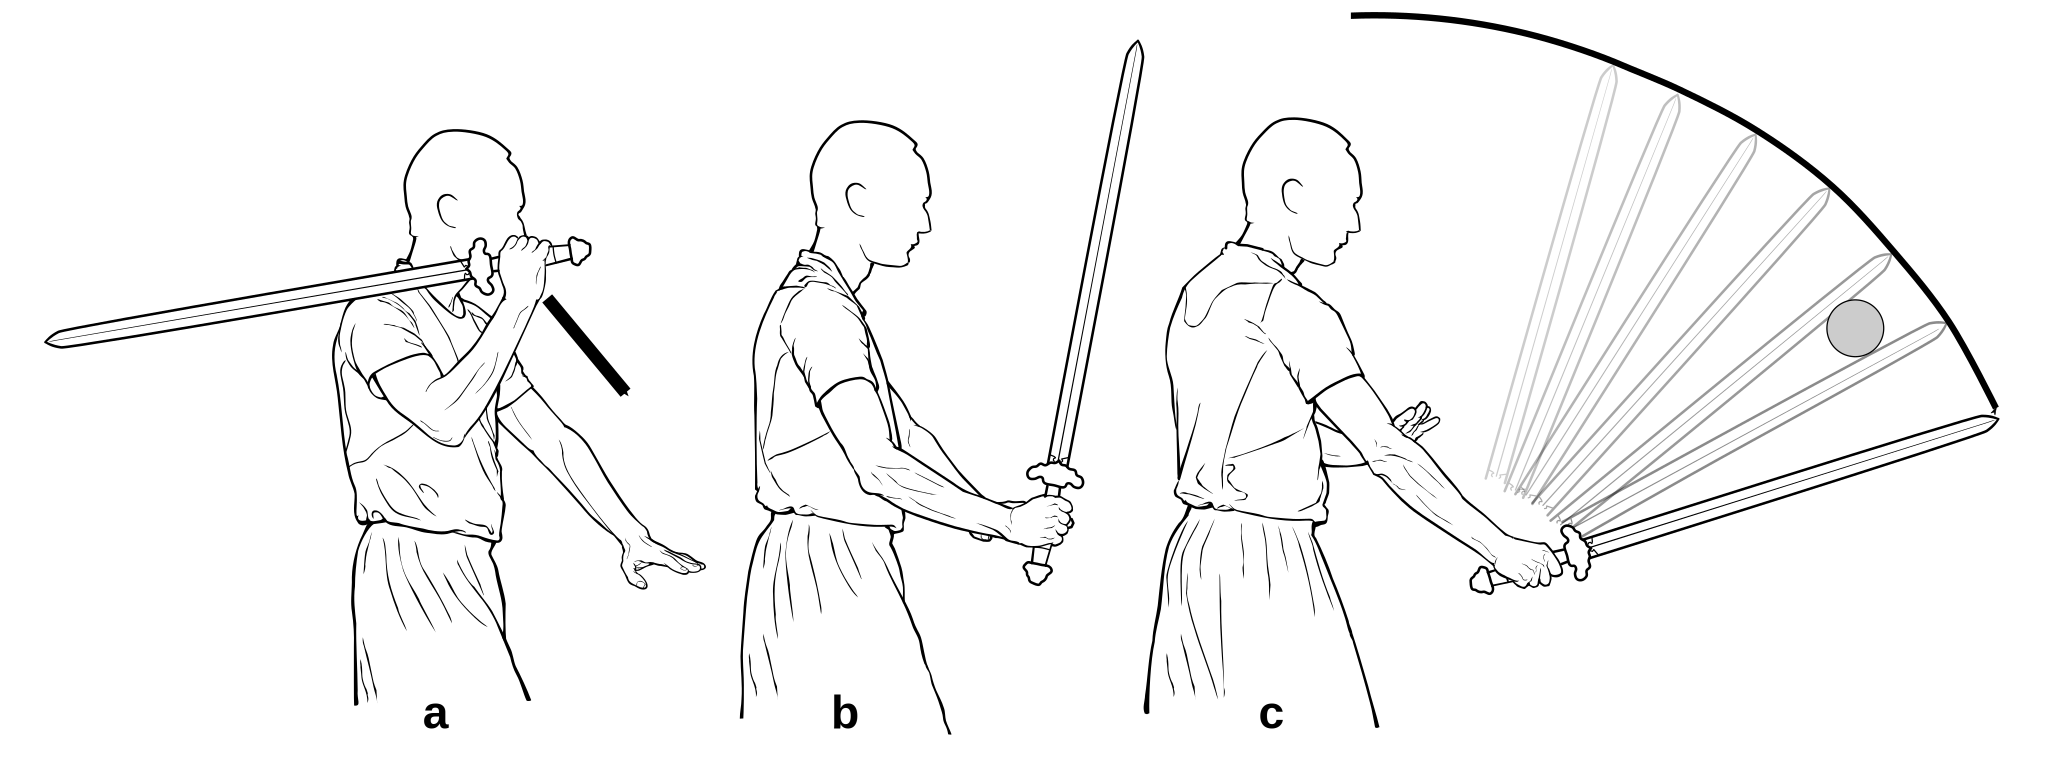
\includegraphics[width=1.00\textwidth]{../../Images/JibenJianfa/Pi/Pi_juxtaposed.pdf}
	\caption[Coupe \Pi{}]{Coupe \Pi{} : (a) Partant d'une position haute de l'épée, la main droite la tire vers le bas pour accélérer la lame; (b) montre la fin de la phase d'accélération, à partir de cet instant, la main n'exercera plus d'action sur la poignée; (c) la main suit la poignée avec juste un contrôle ferme de la trajectoire de l'épée de manière à ce que la lame puisse librement traverser la cible représentée par un cercle gris. Notez que la trajectoire de la pointe n'est pas un cercle mais un arc allongé.}
	\label{fig:pi_cut}
\end{figure}

Il est absolument indispensable que le plat de la lame soit parfaitement aligné avec la trajectoire de la l'épée pour garantir que le poids de la lame soit derrière le tranchant pour le pousser à travers la cible. Si jamais la lame atteignait la cible avec un angle, aussi petit soit-il, elle tendrait à tourner autour de son axe et pourrait rebondir dangereusement au lieu de trancher. Lorsque l'alignement est correct, au contraire, et que la prise est relâchée, la lame pourra traverser la cible de part en part sans retour notable.

Après la coupe, la poignée bute naturellement contre le talon de la main et les doigts resserrent leur prise pour arrêter l'épée dans une position de garde à hauteur de taille, sans aucune tension ni rebond. Grâce à une bonne structure corporelle, l'énergie de l'épée retourne ainsi au corps, aidant le recentrage, et la préparation de la technique suivante.
% !TeX spellcheck = fr_FR
\section{\Hua}
Le verbe \Hua{} \begin{CJK*}{UTF8}{bsmi}劃\end{CJK*} signifie \textit{délimiter}, \textit{tracer}. Ce caractère est aussi une variante du mot désignant un trait dans un caractère chinois.
La partie de gauche de ce caractère étant la clé du pinceau, ces observation suggèrent que cette technique évoque la notion de calligraphie, d'écriture et de dessin.

Le \Yangjia{} \Michuan{} présente la technique \Hua{} emblématique comme une coupe horizontale ou un large mouvement horizontal dans le but de maintenir les adversaires à distance. L'idée est ici de balayer l'espace avec l'épée pour délimiter la zone la plus large possible autour de soi et d'entailler quiconque ose s'approcher.

D'une manière plus générale, les coupes \Hua{} ne sont pas systématiquement horizontales et s'appliquent à différentes distances, depuis des entailles réalisées à longue distance avec la pointe de l'épée, jusqu'à des coupes glissées avec toute la longueur du tranchant à courte distance. Dans tous les cas, les coupes \Hua{} ont pour caractéristique commune le fait que la lame trace progressivement une longue entaille, au contraire de \Pi{} qui fend la cible d'un coup. 

Pour réaliser une coupe \Hua{} à longue distance, l'épée est lancée en avant et, lorsque le bras a presque atteint son extension complète, juste avant que la lame ne frappe la cible, la prise se resserre doucement sur la poignée pour assurer la connexion entre les centres de l'épée et du corps. La rotation continue ainsi à partir de l'épaule tandis que l'épée tire le corps en avant jusqu'à ce que la portée maximale soit atteinte (fig. \ref{fig:hua_cut} a-c). Ensuite, la prise agissant comme un levier, l'inertie de l'épée repousse la poignée contre le talon de la main, engendrant un mouvement vers l'arrière qui génère une coupe glissée et recentre le corps dans une posture de garde (fig. \ref{fig:hua_cut} d-f). 

\begin{figure}[ht]
\centering
	\includegraphics[width=1.00\textwidth]{../../Images/JibenJianfa/Hua/Hua.pdf}
	\caption[Coupe \Hua{}]{Coupe \Hua{} : (a) \'{A} partir d'une position haute de l'épée, (b) la main droite lance le pommeau vers l'avant; (c) montre la fin de la phase active de la technique; (d) à (f) pendant la phase passive, l'inertie de l'épée repousse la main en arrière, réalisant la coupe glissée et recentrant le corps en position.}
	\label{fig:hua_cut}
\end{figure}

\'{A} plus courte distance, la dynamique des coupes \Hua{} utilise moins l'inertie de l'épée mais s'appuie plus sur la structure et le mouvement du corps. Dès que le tranchant est en contact, la coupe est effectuée en pressant le tranchant contre la cible et en tirant l'épée selon une direction parallèle à l'épée, en se déplaçant ou en tournant le corps. Il est parfois possible, en particulier en passant dans le dos de l'adversaire, de réaliser avec le faux tranchant une coupe \Hua{} à courte distance.

En plus d'être une coupe glissée, \Hua{} peut aussi être utilisé pour maintenir des adversaires à distance ou les obliger à réagir de façon à exploiter leur action et prendre le contrôle du rythme. Pour ce faire, on peut lancer une coupe \Hua{} sans toutefois s'engager totalement, ou faire des moulinets tout en avançant. La distance doit dans ce cas est suffisamment courte pour que ces coupes soient clairement perçues comme une menace bien qu'on puisse être légèrement hors de mesure. La distance idéale est à la limite supérieure de la mesure courte, distance à laquelle, bien qu'elle soit incertaine, une touche est tout à fait plausible et l'adversaire ne peut que se sentir obligé de réagir défensivement. Il est important dans ce cas de se préparer à doubler avec une attaque plus engagée ou un contrôle de la lame selon les circonstances. C'est cette seconde intention qui permettra de prendre l'initiative en exploitant l'action de l'adversaire.

En rompant la distance après une attaque infructueuse, il est possible de maintenir l'adversaire à distance avec une série de moulinets que Maître Wang Yennien décrivait également comme étant des coupes \Hua{}. Cette application de la technique correspond parfaitement à la traduction \textit{délimiter} puisqu'elle crée en effet une zone de sécurité empêchant l'adversaire d'entrer et d'attaquer pendant qu'on se place hors de mesure.

% !TeX spellcheck = fr_FR
\section{\Ci{}}
On trouve le mot \Ci{} \begin{CJK*}{UTF8}{bsmi}刺\end{CJK*}, signifiant \textit{estoquer}, \textit{percer}, \textit{poignarder}, dans le \WubeiZhi{} comme terme générique désignant l'ensemble des techniques d'estoc à l'épée. D'autres traités anciens le mentionnent aussi pour décrire les estocs avec diverses armes. 

Dans la tradition du \Yangjia{} \Michuan{}, \Ci{} est défini comme un estoc horizontal ou remontant, poussant la pointe puissamment à travers la cible. 

On réalise généralement la technique formelle en commençant sur le pied droit, pied gauche en avant, soit avec une passe avant (\Ci{} long), soit avec un simple transfert de poids sur le pied gauche (\Ci{} court). Dans le contexte formel des exercices et de la forme, la cible du \Ci{} court est l'abdomen, celle du long est la base de la gorge. En assaut par contre, on peut viser d'autres cibles telles que le torse, ou même le visage.

Que la technique réalisée soit longue ou courte, on commence invariablement par créer dans le corps une structure spiralée connectant le pied gauche et l'épée. Dès que la taille bouge, le bras droit pousse sur la poignée et se lève en un mouvement spiralé qui s'achèvera avec une position d'épée horizontale, sur son plat, le pommeau orienté vers la hanche gauche. Dans le même temps, on transfère le poids sur le pied gauche. La prise de l'épée s'adapte progressivement pour maintenir une connexion ininterrompue entre la main et la poignée, sans aucun angle, permettant de pousser sans effort l'épée vers avant. Cet ajustement permet également d'exercer sur la poignée une action oblique atteignant au delà de la garde le point générant un point pivot dans la pointe de la lame pour la stabiliser\footnote{Voyez le chapitre \ref*{ch:epeechinoise} pour de plus amples détails sur les points pivots.}. 


La passe avant du \Ci{} long permet une portée plus longue. Le bras droit doit être étendu avant d'avancer pour augmenter la précision de l'estoc et placer le corps derrière l'épée, aussi loin que possible du danger. Engager la lame de l'adversaire pour la contrôler avec la garde ou le fort de la lame, permet encore une meilleure protection. 

\begin{figure}[ht]
\centering
	\includegraphics[width=1.00\textwidth]{../../Images/JibenJianfa/Ci/Ci_thrust_arc.pdf}
	\caption[Estoc \Ci{} long]{\`{A} la fin de l'estoc \Ci{} long, l'épée est alignée avec la hanche gauche mais sa pointe est dirigée vers le centre, visant la base de la gorge. La puissance de toute la structure du corps se concentre dans l'épée pour pousser la pointe à travers la cible.}
	\label{fig:ci_thrust}
\end{figure}

Idéalement, le talon droit devrait toucher le sol exactement au moment où la pointe de la lame atteint la cible. Le relâchement de la structure achève alors le pas en poussant la lame au travers de la cible. Il est important de ne pas se laisser tomber dans la jambe droite de manière à conserver une capacité de se retirer rapidement en cas de nécessité. Cela ne signifie toutefois pas qu'on ne doit jamais transférer le poids sur la jambe droite, mais que la polarité vide/plein entre les deux jambes doit être maintenue en toutes circonstances pour éviter la double lourdeur. L'arc de force venant du pied gauche, traversant le dos, spiralant le long du bras droit jusqu'à la pointe de l'épée, et soutenu par la spirale du bras gauche, génère ainsi une structure à la fois puissante et mobile.

% !TeX spellcheck = en_GB
\section{\Duo}
The translation of \Duo{} \begin{CJK*}{UTF8}{bsmi}剁\end{CJK*}, referring to the cooking term \textit{to mince}, somehow suggests repetition and cutting using a part of the blade further away from the tip than \Pi{}. The movement itself is a combination of a forward extension with some sort of shearing, as if using a large cooking knife to mince herbs or vegetables.

In the \Yangjia{} \Michuan{} tradition, the emblematic \Duo{} is performed with both arms extended almost in line with the sword's blade (fig. \ref{fig:duo_full}). 


\begin{figure}[ht]
	\centering
	
	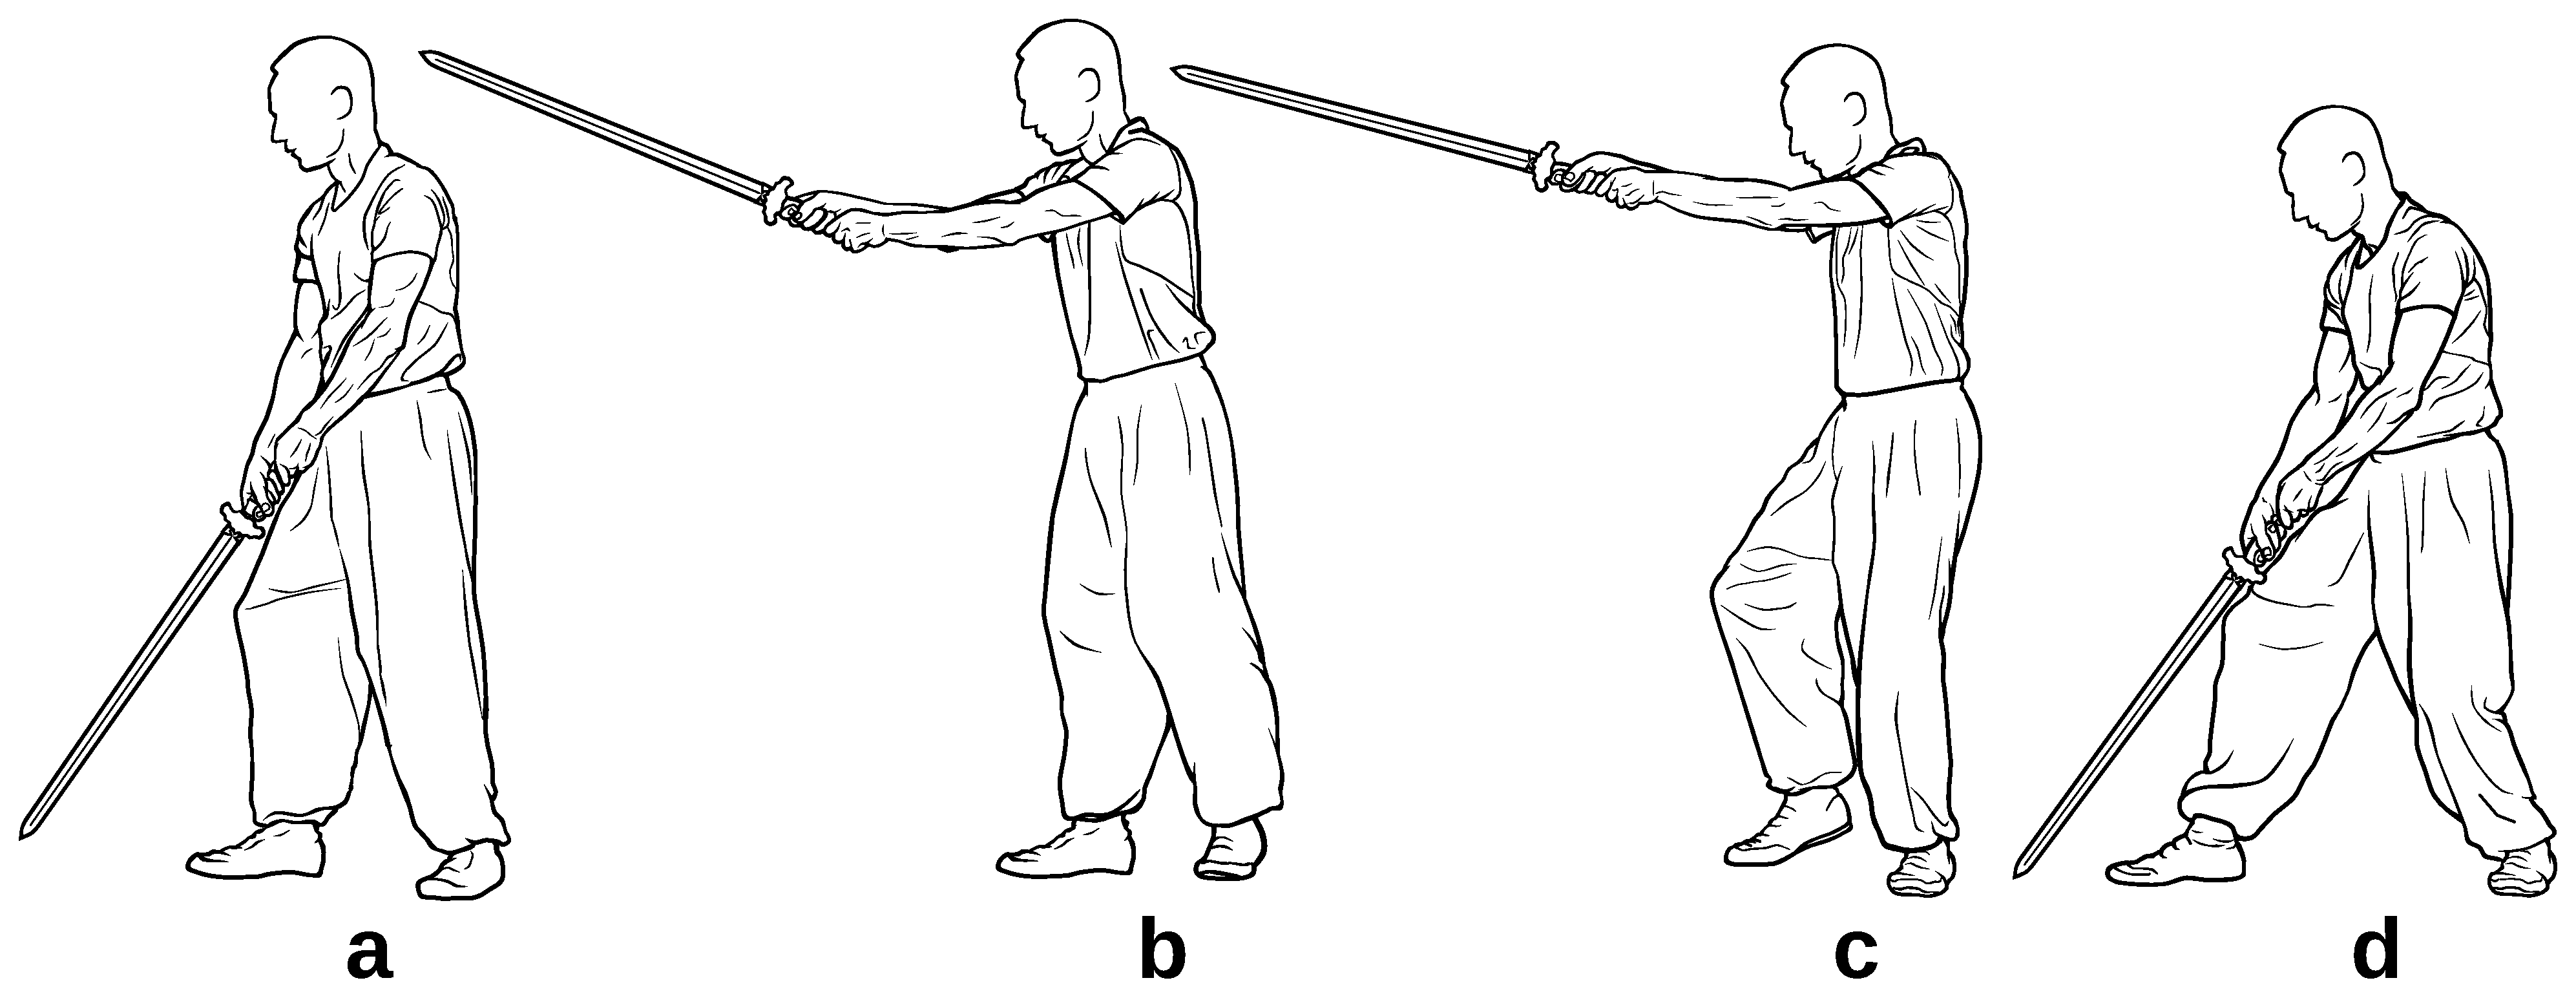
\includegraphics[width=1.00\textwidth]{../../Images/JibenJianfa/Duo/Duo.pdf}
	\caption[Advancing \Duo{}]{\Duo{} in the forward direction. From a low guard (a), raise the sword with a transfer of the weight onto the right foot (b), invert polarity and transfer the weight back onto the left foot (c), drop the sword while sinking in the left leg and advancing the right foot.}
	\label{fig:duo_full}
\end{figure} 

Even though both hands are in contact with the handle,  this should not be mistaken for a true double handed grip of the sword. While raising the sword and advancing, the right hand holds the sword while the left hand provides the structure and power coming from the waist by acting on the pommel along the direction of the blade. The combination of the right hand's passive role with the left hand's action creates a polarity resulting in a movement of the sword perpendicular to the axis of the right arm. When lowering the sword, the roles of both hands are inverted (fig. \ref{fig:duo_detail}). 

\begin{figure}[ht]
	\centering
	
	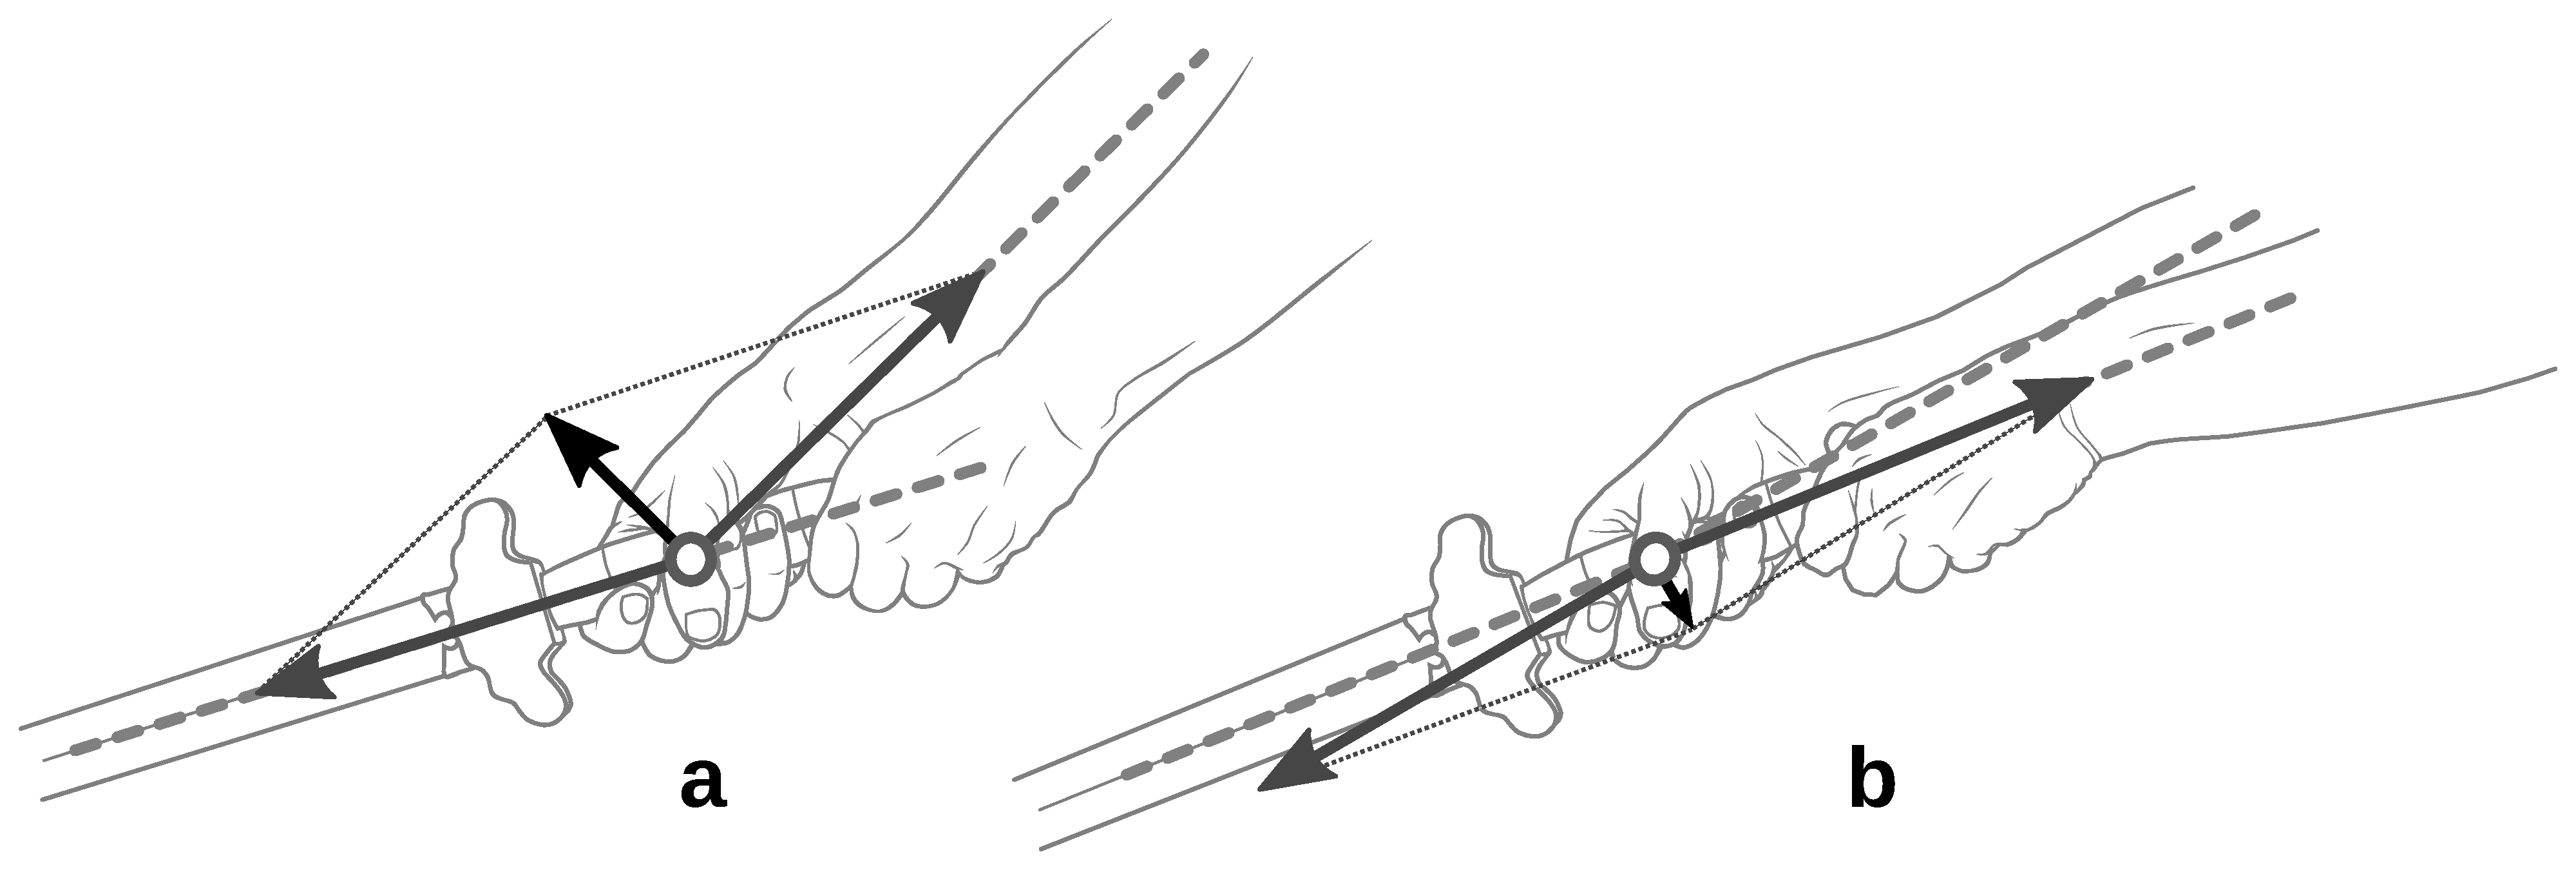
\includegraphics[width=1.00\textwidth]{../../Images/JibenJianfa/Duo/DuoDetail.pdf}
	\caption[Balance of forces in \Duo{}]{(a) To perform a forward rising \Duo{}, the left hand pushes the handle in the direction of the blade tip while the right arm passively balances the pushing force. Due to the angle between the pushing direction and the right arm, the resulting force perpendicular to the right arm pushes the sword upwards.\\
	(b) To perform a forward descending \Duo{}, the right hand pushes the handle while the left arm passively balances this force. The resulting force perpendicular to the left arm, draws the sword downwards.
	}
	\label{fig:duo_detail}
\end{figure} 

The power of the ascending forward \Duo{} thus originates in the weight transfer from the rear leg onto the fore leg, is transmitted to the sword by the left/rear hand with the right/fore hand exactly and passively balancing the forces to effortlessly generate the technique. An effective connexion between the waist and the sword will allow the explosive expression of the \Duo{} technique. 
This method somehow echoes the precepts found in the \JianJing{} stating that, when wielding a double-handed sword, power is first in the waist, then in the rear hand, and finally in the fore hand.

For the retreating \Duo{}, however, the hands play a reversed role: the right hand is active when raising the sword, and passive otherwise. As a rule of thumb, advancing or retreating, the active hand is always the one on the same side as the foot that is moving.

Since, when cooking, herbs are usually minced by cutting downwards, we may argue that the active phase of \Duo{} is the descending one. However, if we examine attentively the actual movement of a kitchen knife when mincing, we may discover that its form when cutting actually corresponds to the rising phase of \Duo{}. The main difference is that the tip of the knife stays down in contact with the table whereas the point of the sword rises up. But, in both cases, the edge follows the same movement relative to the tip. 
However, it is perfectly possible to be active in both phases, the actual passive phase being the transition movement between the ascending and descending parts of the technique. Thus, \Duo{} can be a raising thrust or cut as well as a descending cut, or, combined with \Mo{} energy, an action on the opponent's blade, either ascending to intercept and deflect or descending to shear. 

It is worth noting at this point that, since both hands are in contact with the hilt, the sword is always in line with the axis of the body. This axis is more to the left when we are on our left foot, in the low on-guard position that precedes the ascending forward phase of \Duo{}. Then, during the lifting phase of the movement, the axis is shifting to the right before being transferred back to the left when descending. Therefore, in the deflect/shear application of  \Duo{} in combination with \Mo{}, during the upward interception/deflection, transferring the weight onto the right/forward leg gently pushes the opponent's tip away, allowing the descending shear to naturally aim at the centre of the opponent's sword, deflecting it further to open the way for a hit while preventing any counter attack. 

\fiche{The simplest application of \Duo{} starts with a lower guard as an invitation for the opponent to prepare an attack. We can then engage and deflect with a \Duo{} before placing our riposte or we may take advantage of the explosive nature of the movement and use an offensive \Duo{} to thrust directly during the opponent's preparation.
\Duo{} is often performed in series of two to three movements, not more to avoid predictability, as seen for the double-handed version in the \Kunlun{} form. We can usually identify three periods in these series: The first \Duo{} movement would intercept an incoming attack, either a \Pi{} or a \Hua{} cut from above or a high level \Ci{} thrust.Then, the second one will deflect the opponent's blade to open the way for the third \Duo{} thrust. Of course, this is not a fixed pattern, and the first movement can be followed by any appropriate technique depending on the circumstances. For instance, instead of deflecting, the second step may accompany the opponent's blade to control it while entering to prepare the riposte.}

Although the classic movement is done with two hands, it is also possible to perform a \Duo{} with one hand only. In this case, the heel of the hand plays the same role as the rear hand in the two-handed version while the first three fingers \textemdash{} the index and middle fingers, and the thumb \textemdash{} play the part of the forehand (figure). 

During the ascending phase, the handle of the sword is pushed forwards by the heel of the hand and simultaneously pulled by the first three fingers. Given a good structure in the on-guard position, it is then possible, even with only one hand, to swiftly and effortlessly raise the sword from a low to a high position, for thrusting or engaging.  
\fiche{When descending, the fore fingers relax their grip while the ring and little fingers are tightened to pull the handle. Some intention should be put at the base of the index to gently push the handle downwards in the forward direction. The resulting structure allows to capture and deflect the centre of the opponent's sword by shearing or to perform a powerful cut while retreating.}
The alignment of the sword is quite similar to the two-handed version, with the tip of the blade in line with the body axis. However, the structure is not as strong as in the two-handed \Duo{} and, as a result, the shearing actions are not as powerful. However, this version of the movement is useful for quickly engaging the opponent's blade or a sudden attack from a lower guard. 

\fiche{
These actions can be chained, as in the \Kunlun{} sword form, by two or three, first intercepting the opponent's blade before deflecting and hitting with a double or treble shearing. 
the polarity between the hands allows the crossed links between hand and foot. 
}
% !TeX spellcheck = fr_FR
\section{\Liao}
\Liao{} \begin{CJK*}{UTF8}{bsmi}撩\end{CJK*} est une coupe montante.
% !TeX spellcheck = en_GB
\section{\Zha}
\Zha{} \begin{CJK*}{UTF8}{bsmi}扎\end{CJK*} is a downward thrust.
\fiche{
	spiralling arc on the outside, from the foot to the point, passing through the back and the outside of the arm and along the true edge. The back is stretched and the breast is relaxed. There is a connection between the foot and the point. The weight of the body and the rotation of the waist inwards will generate the thrust. The arm extends in coordination but not excessively
	The unarmed hand can control the opponent's arm, especially when chained after parrying \Liao{}.
	
	check the translation and make sure to use the simplified character
	translation: set up (a tent)
	
	rem: there exists another character which is simplified into this one and is pronounced at the first tone and means
}
% !TeX spellcheck = en_GB
\section{\Mo}
\Mo{} \begin{CJK*}{UTF8}{bsmi}抹\end{CJK*} encompasses all the techniques that take control of the centre of the opponent's blade.
\fiche{
	principle of controlling, deflecting, directing, listening
	the intention is located closer to the forte
	
	translation: put, spread (butter, etc.), wipe
	use the simple character
	
	maybe related to a variety of techniques used to parry, such as wash, shave, shear. ..
	
	radical mo is probably phonetical although it means powder (waste, residuals)
	
	sliding contact of the blades (wipe) with a deflecting action of control thanks to the opposition of the forte against the feeble of the opponent,  this is found in blade capture (coulé, opposition, ...) or the control of the blade during attacks
	
	lateral and aiming at the centre of the opponent's blade, if only lateral we give way to transformation by the opponent and we don't have control of their blade. 
	
	relationship with feeling through the blade and cover
	during parries, absorption, deflection, protection
}

% !TeX spellcheck = fr_FR
\section{\Tiao}
\Tiao{} \begin{CJK*}{UTF8}{bsmi}挑\end{CJK*} est une coupe rapide réalisée avec le faux tranchant.

% !TeX spellcheck = fr_FR
\section{\Dian}
\Dian{} \begin{CJK*}{UTF8}{bsmi}點\end{CJK*} est un estoc rapide ou une coupe légère réalisée avec l'extrémité de la lame.

\fiche{
\section{What makes a cut effective? }
relaxation, blade alignment
distance
must travel through the target
split or slice

\section{ What makes a thrust effective?}
point control, see pivot points in chapter 2
distance
no need for more than a few centimetres in the target to reach a vital organ
}

% !TeX spellcheck = en_GB
\chapter{Footwork}\label{ch:footwork}

This chapter will discuss the footwork in \Taijijian{}.
\part{\Taijijian{} fencing}
% !TeX spellcheck = en_GB
\chapter{Time and Distance}\label{ch:distancetime}

Like for any martial art, time and distance are most essential notions to fencing.
It is only by mastering them that one may hope to become a truly proficient fencer.

Intricately intertwined, these two concepts are not absolute nor fixed notions though and bear all but no relation with actual physical dimensions.
While they do help describing and objectively commenting fencing actions,
they also encompass the sense of time and distance in a context of confrontation, that is to say the perception that the opponents have of their relative capacities of action.
As such, time and distance are central to fencing tactics and strategy.

\section{Fencing time} \index{fencing time}
\emph{Fencing time} is a unit of time defined as the duration of a simple action: a step, a cut, a thrust, a parry, etc.\index{simple actions}
The number of time units taken by a combined action is the number of consecutive simple actions that compose it, simultaneous simple actions counting for one unit of time only.
For example, one step while parrying followed by a riposte would sum up to two time units in all.

Fencing time is not related to actual clock time, it is not a definite span of time since the actual duration of a simple action will depend upon the speed at which it is executed.
Fencing time is rather related to the notion of commitment in an action associated with an underlying intent.\index{intention}\index{transformation}
As long as the fencer is not fully engaged in his action, he may still transform and change his intent during the same unit of time.
It is only after full commitment that it becomes impossible to interrupt the course of the ongoing action and change one's mind during the same fencing time.
This does not mean though that an action must necessarily be led to its term as soon as it has been initiated but that transformations take more time when the intention is fully engaged.

This very important tactical notion is used in feints and false attacks.
As we shall see further, when feinting, full commitment is not sought but the fake strike must be convincing enough to compel the opponent to get fully involved in parrying what he thinks to be an attack.
It is then possible to modify our initial action during the same time and launch the true attack while the opponent, sticking to his first reaction, is baffled.
As a general rule, it should be avoided to engage in action too early so as to preserve for as long as possible a capacity to transform and adapt effectively to the opponent's reactions.

Fencing time may thus be seen as a useful theoretical notion for assessing the fencers' current ability for initiative, transformation or response during actions. 
It helps to formalise the course of simple actions when studying a \emph{phrase d'arme}, no matter how fast or slow it is performed and assuming that both opponents are equally fast.
Of course, in real life, some fencers are faster than others but actually, speed does not matter. Only tempo is important: what really counts is the right action at the right time.
It is always possible to compensate for a lesser speed with the effective use of techniques and tactics, and above all, by mastering rhythm.\index{rhythm}
A faster fencer may loose his advantage if he is forced by a proficient opponent to use more fencing times for his actions.
This is sometimes adopted as a strategy by some fencers who keep their opponent in a constant state of urgency while allowing themselves to take their time.
Whether they do so by maintaining a permanent threat against their opponent or by always stepping out of his lines of attack, they impose their own rhythm on the fight and do not allow their opponent to regain the initiative.
To achieve this goal however, it is essential for them to stay connected to their opponent and that every single move and menace perfectly fits his reactions.
In other words, the rhythm of the fight is actually a combination of the rhythms of both opponents.
Although, the rhythm of one fencer may take precedence over the other's it never does so independently: connection and relationship are essential.

The ability to grasp and match the rhythm of our opponent while concealing our own is therefore fundamental to seize the right moment and gain an advantage.
It is essential to maintain a constant awareness of the opponent's moves and not to get trapped into heedless anticipation by misleading regular rhythm patterns. 
Great care should be paid too not to embrace too regular a rhythm that would consequently be easily predictable by the opponent. 
Controlling rhythm does imply a relaxed state of mind ensuring we are constantly ready to adapt to the situation and transform it to our advantage by responding to the opponent's moves unexpectedly.
More than quick reactions though \textemdash{} haste should not be mistaken for speed \textemdash{} this is definitely a question of being on the edge of a perpetual present, letting the past flow away and the future happen without clinging to any premeditated technique.

\section{Distance and measure} \index{distance}
Just as fencing time does not actually represent an objective span of time, the effect of the distance between the two opponents on their respective ability to strike each other is more important here than their actual distance.
We thus define measure \index{measure} as the distance range within which it is possible to hit the opponent in one fencing time.
In other words, it is a distance close enough for not requiring more than one step to strike.
If at least two steps are necessary, we are said to be out of measure.

On this basis, three in-measure distances may be defined:
\begin{enumerate}
\item \emph{Guard distance} or \emph{long measure}: one step is required for striking. This is the most usual distance in free play as it offers a good compromise between a protective attitude and a more pressing one.
\item \emph{Reach distance} or \emph{short measure}: at this distance, it is possible to strike with the appropriate section of the blade without having to step forward nor backward.
\item \emph{Close distance}: this distance is too short to use the blade effectively, only close combat techniques can be used such as kicking, punching, grappling, etc.
\end{enumerate}

But there is much more to measure than distance.
Measure is influenced indeed by the fencers' stances and their respective angles of attack.
The guard and foot position determine the range that can be covered by the sword during one fencing time with simple actions: step, weight transfer, arm and body rotation. \index{simple actions}
Whether the target being aimed at actually lies or not within this range and may be reached in one time by an effective cut or thrust will in turn mainly depend upon the angle of attack and the opponent's cover.

It should be reminded that both the angle of attack and the sword's range must be considered here not only in the horizontal plane but in three dimensions, the longest distance being attained with the arm fully extended horizontally at shoulder level.
Thus, in any situation, the closest targets are those approximately lying at shoulder's height, that is, most of the time, the upper chest and the throat.
Lower targets may be reached by stepping forward but also by crouching or leaning so as to lower the shoulder down to target level.

Figure \ref{fig:distance_stance} shows how the sword's range is affected by the fencer's stance and stepping as well as by the height of the target.

\begin{figure}[h]
\centering
	
\includegraphics[width=1.0\textwidth]{../../Images/DistanceTime/distance_stance.pdf}
	\caption[Stance and measure]{Some examples of stances and their thrusting range.\\
	The leftmost column shows the distance reached by extending the arm from the initial guard position (drawn in grey). This distance is slightly longer with the right foot forward (bottom figure) because of the larger turning range of the body pushing the sword further. This can also be observed on the guard position which extends slightly further with the right foot in front. The same remark holds for the middle column showing the range attained by extending the arm and closing the step. This difference is smaller though because of the shorter distance between the feet.\\
	The top right figure shows the maximum range that can be reached with a thrust. Thus, the upper grey box represents the length of the measure when starting with the left foot forward. Thanks to the shifting of the axis to the left foot and the subsequent passing step, this measure is longer than when starting directly with the right foot forward.\\
	In the bottom right figure, the portion of circle represents the vertical range of the sword when standing up without stepping. Even though they may be at the same horizontal distance from the body axis, lower targets may none the less be out of reach unless crouching so as to bring the shoulder at their level.\\
	All figures are drawn to scale.}
	\label{fig:distance_stance}
\end{figure}

Fencing being dynamic by nature, measure must be further accounted for in an ever changing context and may vary dramatically with every single move of the opponents.
As stepping away from the target increases distance, one may be close enough to be statically in measure, but may be at the same time out of measure if evaluated dynamically.
The combination of time and distance reduces or increases the relative duration of of fencing of fencing time units for each opponent depending on whether their steps bring them closer to or further from their target.

%\begin{figure}[ht]
%\centering
%	\includegraphics[width=0.69\textwidth]{../../Images/EmptyFig.pdf}
%	\caption[Motion and measure]{Motion and measure}
%	\label{fig:distance_motion}
%\end{figure}

The concept of measure is not symmetrical indeed and the opponents are not necessarily within the same measure relatively to each other due to different stances, relative moves or respective angles of attack. 
%As shown in figure \ref{fig:distance_motion}, 
A fencer may thus leverage the asymmetry of measure by stepping towards a direction and from an angle that would dynamically keep his opponent out of measure while simultaneously allowing himself to hit.
\FloatBarrier

This is actually a key to efficient \Taiji{} fencing: the opponent is overcome by the appropriate move at the appropriate time and distance, not by a greater speed.
The principles are respected and the fencer's moves can thus be calm and his mind serene.
It is therefore fundamental to develop an ability to instantly perceive one's own measure as well as the capacity of the opponent to hit so as to constantly adapt to the opponent's moves and strike him on the spot when it is possible to do so while keeping away from his threat.

\section{Drills and exercises}
The following drills and exercises will allow you to apprehend and practice the sense of distance and time.

\subsection{Still target}
This drill is adapted from the one called \emph{tirer au mur} in western fencing.
It consists in aiming thrusts or cuts at a non-moving target.

Take place in front of the target at a long-measure distance, draw a thrust or a cut at the target with one step. 

Repeat this drill starting from various foot positions until you have a good grasp of the long measure in all stances.

Then, you may try yourself at the dynamic version of this drill.
Instead of starting directly in measure, start now from a longer distance requiring more than one step to bring you in short measure.
Approach and strike at the target without interruption, while stepping.

Practise this drill slowly at first and increase your speed gradually, but do not go faster as long as you need to reduce your speed or mark a stop before aiming at the target.
The goal here is to acquire the capacity to evaluate the distance while approaching the target and hit as soon as you are at the appropriate distance.

To increase difficulty, you may also vary the angles of attack and approach in sinuous lines.

Ideally, in order to avoid hard shocks and account for penetration of the blade, the target should yield to hits.
Clothes-pegs on a clothes-line hung at throat level make pretty suitable targets in this regard.

\subsection{Moving target}
This drill is adapted from Olivier Delannoy.
It should be practised with secured blades exclusively and the partner holding the target should at least wear a fencing mask.
You will also need a portable target such as a wooden plank with handles, a table tennis racket or a boxing pad.

The partner holding the target moves around facing the partner carrying the sword, keeping the target turned toward the floor.
The latter follows the stepping of the former, trying to stay in measure.
The target holder may raise the target at any time.
At this signal, his partner must draw a thrust at the target if he is at the appropriate distance.

With a boxing pad or a racket, it is also possible to practice this drill with cuts.

\subsection{Double threat}
%It was inspired by a drill proposed by Keith Farell.
This exercise should be practised very slowly with secured blades and fencing masks.
Full protective gear would be required should the partners decide to play faster.

One partner assumes any stance or guard that may please him and his two partners take a threatening position in measure.

The first partner must then find a way to evade the threats and stay out of the measure of both his partners while hitting at least one of them.

Both threatening partners should stay still for the whole duration of the exercise.
However, in a variant of this drill, they may move slowly, at the same pace as the first partner, to check he really is at a safe distance.

The partners should always take their time in this exercise so as to be able to analyse the situation and practice safely. 

This exercise may be practised with more than three partners.

\subsection{Multiple attackers}
This exercise should be performed imperatively with secured blades and full protective gear.

One partner must defend against the continuous attacks from several partners.
His goal is to deal with as many successive attacks as he can.

Each attack must be launched as soon as the defender has parried the previous one and riposted, but not before.

Attackers should fully engage in their attacks and not try to adapt to the defender's parries.

When responding to an attack, the defender must keep control of his distance to other attackers in order to maintain them out of measure and thus ensure he has enough time to react to their attacks.

\newsavebox{\todoDistance}
\sbox{\todoDistance}{
Include the following in the first figure caption.

This kind of stepping is encountered several times in the Kunlun sword routine, accompanied by an extension of the arm, under the form of a chasing step or a half step preparing a subsequent passing step of the left foot.
On the other hand, when on the left

When in regular stance, right foot forward with the weight on the left foot, advancing brings the weight above the right foot, thus gaining the few inches that were mising to reach the target.
When in crossed stance for instance, a forward passing step of the right foot will bring the whole right side of the body forward, and the sword along with it.
It will thus be possible to hit in one time from much further than if starting with the right foot in front since a passing step of the left foot will not as much allow the sword to simultaneously near the target (see figure \ref{fig:distance_passing_step}).
At close distance, a backward passing step into the crossed stance would bring the sword tip back in front of the opponent's body and ready to thrust.
Figure with different stances and hitting range: better than obcure explanations in the text.


...
? paragraph on strategy and tactics and time and distance
no, the reverse: a paragraph on time and distance in the chapter about strategy

A tall fencer will be in measure at a larger distance, just as someone who has a longer blade. 
Their close distance will also be larger though, which may not be an advantage.

For instance, by assuming an opposite guard, it is possible be at reach distance inside the guard of the opponent who consequently is at close distance: we can thrust at our opponent whereas he cannot use his weapon effectively.
An evident strategy based on these premises consists in progressing gradually towards the reach distance while maintaining the opponent out of measure or at worse in his guard distance.

When in guard distance, mobility should be favoured in order to explore the situation and search for openings in the opponent's guard where it would be possible to enter and hit in one time. The uncovered side is mobile and can dodge if the opponent works his way around our guard and attacks. Mobility is most important so as not to offer a still and easy to reach target.
Ideally, at guard distance, a complete back stance should place us out of measure. Thus, this distance provides a good compromise between safety and the capacity to hit.
In reach distance, we should try and find an opportunity to hit by approaching as much as necessary while keeping the body as far as possible and above all, covered and well protected.
}

% !TeX spellcheck = en_GB
\chapter{The lines}\label{ch:lines}

This chapter will discuss the concept of lines in fencing.

There are four lines referring to the position of the blade relative to the opponent's sword while engaging, attacking or parrying: inside, outside, above or below.

% !TeX spellcheck = en_GB
\chapter{The guards}\label{ch:guards}

A guard is any posture that may be used to protect oneself while preparing an attack.

This chapter will present the nine guards that can be identified in the \Yangjia{} \Michuan{} \Taijijian{} \Kunlun{} sword form.
These guards are not part of the traditional transmission. They are postures frequently encountered in the form that may correspond to the above definition of a guard.
% !TeX spellcheck = en_GB
\chapter{Free play}\label{ch:sparring}

This chapter will discuss the various aspects of free sparring, including technical, tactical and strategic considerations.
% !TeX spellcheck = fr_FR
\chapter{Applications martiales}\label{ch:applications}

Ce chapitre présentera une sélections d'applications martiales de la forme d'épée \Kunlun{} du \Yangjia{} \Michuan{} \Taijijian{}. Ces illustrations seront sélectionnées pour illustrer les concepts discutés dans les autres chapitres.
\part{\Taiji{} principles}
% !TeX spellcheck = en_GB
\chapter{The \Taiji{} classics}\label{ch:classics}

The \Taiji{} classics are texts written at the end of the XIX\textsuperscript{th} century and composing a corpus common to all styles of \Taijiquan{}.

This chapter will, within the scope of fencing, discuss the principles of \Taiji{} described in these text and that will be developed further in the following chapters.
% !TeX spellcheck = fr_FR
\chapter{Fluidité et transformation}\label{ch:transformation}

La fluidité et la transformation sont des points fondamentaux du \Taijiquan{} et par conséquent du \Taijijian{}.
Ils découlent de l'application des principes décrits dans les textes classiques comme le relâchement, la compréhension du \Yin/\Yang{}, etc. 
% !TeX spellcheck = fr_FR
\chapter{Les énergies Jing}\label{ch:jing}

Ce chapitre discutera des différentes énergies Jing: Ding jing, Dong jing, Hua jing et Fa jing.
% !TeX spellcheck = en_GB
\chapter{The \Si{} \Yao}\label{ch:siyao}

This chapter will present the \Si{} \Yao{} (\Zhan, \Nian, \Lian, \Sui) considered from a fencing point of view\ldots

% !TeX spellcheck = fr_FR
\chapter{Le \Yi}\label{ch:yi}

Ce chapitre présentera les différents aspects du \Yi{} in \Taijijian{} de la pratique de la forme à l'assaut libre\ldots
\part{Appendices}
\appendix
% !TeX spellcheck = fr_FR
\chapter{La forme d'épée \Kunlun{}}\label{ch:kunlun}

Un bref aperçu de cette forme.
% !TeX spellcheck = en_GB
\chapter{Glossary}\label{ch:glossary}
%\printglossaries
\backmatter
\printindex
\end{document}